%------------------------------------------------------------------------------
%
% TeC7 ハードウェアマニュアル
%
%------------------------------------------------------------------------------
\documentclass[a4paper,11pt,twocolumn]{ltjsbook}      % lualatex の場合
\usepackage{mySty}
\newcommand{\ver}{Ver. 2.0.0}
%------------------------------------------------------------------------------
% はじまり
\begin{document}
\frontmatter
%------------------------------------------------------------------------------
% 表紙
\title{{\tecS} ハードウェアマニュアル \ver}
\author{徳山工業高等専門学校\\情報電子工学科}
\date{}
\maketitle

%------------------------------------------------------------------------------
% 著作権表示
\thispagestyle{empty}
\onecolumn
~
\vfill
\begin{flushleft}
Copyright \copyright ~~ 2019 - 2022 by \\
Dept. of Computer Science and Electronic Engineering, \\
Tokuyama College of Technology, JAPAN
\end{flushleft}

\vspace{0.8cm}
本ドキュメントはCC-BY-SA 4.0 ライセンスによって許諾されています。

% 本ドキュメントは
% CC-BY-SA 3.0 de ライセンス,
% CC-BY-SA 4.0 ライセンス
% で許諾された著作物を含みます.

% (CC-BY-SA 3.0 de ライセンス全文は
% \url{https://creativecommons.org/licenses/by-sa/3.0/de/}で,
% CC-BY-SA 4.0 ライセンス全文は
% \url{https://creativecommons.org/licenses/by-sa/4.0/deed.ja}で確認できます.)

%------------------------------------------------------------------------------
% 目次
\setcounter{tocdepth}{2}
\tableofcontents

% 本文
%\twocolumn
\mainmatter

\chapter{概要}
このマニュアルでは{\tecS}のハードウェアとIPLプログラムについて解説を行う.

%----------------------------------
\section{\tecS}
\tecS は,
内部に{\tec}と{\tac}の二つのコンピュータを内蔵したマイコンボードである.

\begin{description}
\item[\tec]
  高校生や高専の低学年の学生が,ノイマン型コンピュータの
  動作原理を学ぶために開発された8ビットコンピュータである.
  コンソールパネルを用いて,
  二進数で機械語プログラミングを体験することができる.
  {\tec}については,
  「TeC教科書」\footnote{
    \url{https://github.com/tctsigemura/TecTextBook/raw/master/tec.pdf}}
  に詳しい説明がある.
\item[\tac]
  大学生や高専の高学年の学生が
  オペレーティングシステムやコンパイラを学習する際に,
  ターゲットとなるコンピュータのサンプルとして
  開発した16ビットコンピュータである.
  本マニュアルは,
  主に{\tac}として使用する際の{\tecS}について解説する.
\end{description}

%----------------------------------
\section{{\tecS}の外観}

\figref{TeC7Photo}に{\tecS}の写真を示す.
{\tecS}は一枚のプリント基板に実装されている.
以下に基板の主要な部品などを紹介する.

\begin{description}
\item[コンソールパネル]
  ユーザはコンソールパネルを用いて,
  {\tec}または{\tac}のCPUレジスタやメモリの内容を読み書きしたり,
  プログラムを機械語命令単位でステップ実行したりすることができる.
  つまり,コンソールはハードウェア仕掛けのデバッガである.
  {\tec}では機械語プログラムのデバッグに,
  {\tac}ではオペレーティングシステムのデバッグに使用する.
  オペレーティングシステムのカーネル内部まで,
  ステップ実行しながらデバッグすることが可能である.
\item[JTAGコネクタ]
  FPGAを設定(コンフィグ)する設計データを書き込むために使用する.
  プリント基板上でFPGAとフラッシュメモリからなるJTAGチェインを構成しており,
  JTAGコネクタからFPGAとフラッシュメモリにアクセスすることができる.
\item[スピーカ]
  コンソールを操作した際に操作音を発生する.
  {\tec}は電子オルゴールプログラム等で使用することもできる.
\item[フラッシュメモリ]
  電源が遮断されても内容が消えないメモリである.
  {\tecS}に電源が投入された時,
  フラッシュメモリからFPGAコンフィグ用のデータが読み出される.
  内容はJTAGコネクタから書き換えることができる.
  使用している部品は,Xilinx XCF04S である.
\item[マイクロSDスロット]
  {\tac}の二次記憶装置としてマイクロSDを使用することができる.
\item[電源(USB)コネクタ]
  電源を供給するために使用する.
  また,FT232RLと接続してあるのでPCとシリアル通信をすることも可能である.
\item[FT232RL]
  PCとUSBで接続してシリアル通信をするためのICである.
\item[クロックIC]
  9.8304MHzのクロック信号を出力する水晶発振器である.
  FPGAにクロック信号を供給する.
\item[FPGA]
  {\tec},{\tac}のCPU,メモリ等,全ての主要な論理回路を内蔵する.
  使用しているFPGAは,Xilinx Spartan-6 XC6SLX9 である.
\item[RN4020]
  BLE(Bluetooth Low Energy)規格の通信モジュールである.
  FT232RLと同様な通信をBluetooth経由で行うことができる\footnote{
    通信相手には
    BlueTerminal(\url{https://github.com/tctsigemura/BlueTerminal})
    をインストールする必要がある.}.
  bバージョン以降の{\tecS}に実装されている.
\item[ジャンパ]
  {\tecS}を{\tec}として使用するか,{\tac}として使用するかを決める.
  その他に,Bluetoothモジュールのリセットや,
  デモンストレーション機能の呼び出しにも使用できる.
\end{description}

\myfigure{tbp}{width=\columnwidth}{Fig/kakubu.pdf}{TeC7の写真}{TeC7Photo}


%----------------------------------
\section{{\tecS}の内部構造}

\figref{TeC7Blk}に{\tecS}のブロック図を示す.
図中央の灰色の大きな長方形はFPGAを表しており,
主要な論理回路は全てFPGAに内蔵されていることが分かる.
FPGA内部の回路はVHDLで記述されている.
{\tecS}の回路を記述したVHDLのソースコードはGitHub\footnote{
\url{https://github.com/tctsigemura/TeC7/tree/master/VHDL}}
に公開してある.
緑色の長方形はプリント基板上に実装されたFPGA以外の部品である.
基板の回路図を付録\ref{appTac},\figref{TeC7Pcb}に示す.
以下では,\figref{TeC7Blk}を参照しながら{\tecS}の回路構成の概要を説明する.

\myfigure{tbp}{scale=.6}{Fig/TeC7.pdf}{TeC7のブロック図}{TeC7Blk}

\subsection{クロックとリセット}
DCMは,外部から供給される9.8304MHzのクロック信号から,
Spartan-6のDCM(Digital Clock Manager)を用いて,
{\tec}用の2.4576MHz,
{\tac}用の49.152MHzクロック信号を生成する.
DCMは電源投入後,クロック出力が安定すると\texttt{i\_locked}を`1'にする.

\texttt{i\_locked}が`1'になるとMODEはジャンパの設定を読み取り
結果を\texttt{i\_mode}に出力する.
ジャンパの読み取りが完了すると,
\texttt{i\_reset\_tec}と\texttt{i\_reset\_tac}が`1'になり,
{\tec}と{\tac}が動作を開始する.

\begin{mytable}{btp}{\texttt{i\_mode}の値と意味}{mode}
  \begin{tabular}{ c | l }\hline\hline
    \texttt{i\_mode} & \multicolumn{1}{|c}{意 味} \\\hline
    \texttt{000} & TeCモード({\tecS}が{\tec}として動作) \\
    \texttt{001} & TaCモード({\tecS}が{\tac}として動作) \\
    \texttt{010} & DEMO1モード(電子オルゴールプログラム入力済みのTeCモード)\\
    \texttt{011} & DEMO2モード(演奏データ入力済みのDEMO1モード)\\
    \texttt{111} & リセット(RN4020を工場出荷時の状態に戻す) \\
  \end{tabular}
\end{mytable}

\subsection{動作モード}
\label{tec7mode}
\texttt{i\_mode}の値により{\tecS}の動作モードが決まる.
\texttt{i\_mode}の値と動作モードの対応を\tabref{mode}に示す.

\begin{itemize}
\item 「TeCモード」,「DEMO1モード」,「DEMO2モード」では,
  {\tec}がコンソールと接続される.
  その様子を\figref{TeC7Blk}で確認する.
  図中の``TeC''が{\tec}コンピュータである.
  この内部に,{\tec}のCPUや主記憶,入出力装置などの回路が組み込まれている.
  \texttt{i\_mode}の値が\texttt{001}(TaCモード),
  \texttt{111}(リセットモード)以外の場合,
  図中のデマルチプレクサ(DMUX)とマルチプレクサ(MUX2)が切り替わり
  {\tec}とコンソールが接続される.
  \texttt{i\_mode}の値が「DEMOモード」の場合は,
  {\tec}のメモリに予め電子オルゴールプログラムが入力された状態になる.
\item 「TaCモード」では,{\tac}がコンソールと接続される.
  図中の``TaC''が{\tac}コンピュータである.
  \texttt{i\_mode}の値が\texttt{001}(TaCモード)の場合は,
  {\tac}にコンソールが接続される.
\item 「リセットモード」では,{\tec}も{\tac}もコンソールに接続されない.
\end{itemize}

{\tec}は「TaCモード」では停止したままになる.
一方で{\tac}は\texttt{i\_mode}の値に関係なくIPLプログラムの実行を開始する.
IPLがモードに対応した動作を行う.

\subsection{{\tac}による{\tec}の補助}
\label{tec7assist}
{\tec}のシリアル入出力(\texttt{i\_tec\_rxd/txd})は{\tac}に接続されており,
「TeCモード」では{\tac}がシリアル入出力の中継装置の役割を担う.
通常,{\tac}はシリアル入出力をFT232RLに中継する.
しかし,RN4020がBluetooth接続を確立した場合は,
FT232RLとRN4020の両方に中継するようになる.
{\tec}は{\tecS}がUSBとBluetoothのどちらで
PCに接続されているのか知る必要がない.

通常,図中の``MUX1''はコンソールを``DMUX''に接続している.
「TeCモード」時に,シリアル通信で受信した内容がTWRITEプログラム\footnote{
\texttt{Util--}(\url{https://github.com/tctsigemura/Util--})に含まれる
プログラム書き込みツールのこと.}のものなら,
通信を中継している{\tac}が``MUX1''を切り換え{\tec}のコンソールを操作し,
受信したプログラムを{\tec}のメモリに書き込む.
この機能は{\tac}のIPLプログラムに組み込まれている.

%----------------------------------
\section{{\tec}の内部構造}

\figref{TeCBlk}に{\tec}のブロック図を示す.
この図は,\figref{TeC7Blk}の``{\tec}''ブロックの内部を表している.

\myfigure{tbp}{scale=.56}{Fig/TeC.pdf}{TeCのブロック図}{TeCBlk}

\subsection{CPU,メモリ,入出力装置}
CPUとメモリや入出力装置はバスを介して接続されている.
入出力装置には,シリアル入出力(SIO),
入出力ポート(PIO),タイマー,A/Dコンバータの機能が含まれる.
SIOはTaCに接続されており,通信データはTaCがFT232RLやRN4020に中継する.
コンソールのデータSWやスピーカは入出力装置としても使用することができる.

\subsection{コンソール}
コンソールは,CPUとメモリに専用の回路で接続されている.
完全にハードウェア制御で動作するので,
プログラム実行中でも操作が可能である.

\subsection{割り込みコントローラ}
割り込みコントローラは,
コンソール,入出力装置から発生する四種類の割り込みをCPUに伝える.
CPUが割り込み認識サイクルに入ったらバスに割り込み番号を出力する.

%----------------------------------
\section{{\tac}の内部構造}

\figref{TaCBlk}に{\tac}のブロック図を示す.
この図は,\figref{TeC7Blk}の``{\tac}''ブロックの内部を表している.

\myfigure{tbp}{scale=.7}{Fig/TaC.pdf}{TaCのブロック図}{TaCBlk}

\subsection{CPU}
CPUは,バスを通してメモリは入出力と接続される.
コンソールからのStop信号が入力されている間はCPUは命令実行を停止する.
CPUがHalt機械語命令を実行した場合は,コンソールにHalt信号を出力する.

\subsection{コンソール}
コンソールのSWやLED,SPKを接続するブロックである.

コンソールは,CPUが命令実行を停止している間だけ機能する.
CPUが命令実行を開始するとコンソールの表示は変化しなくなる.
その間は,プログラムから入出力装置として使用することができる.

\subsection{割り込みコントローラ}
マイクロSDホストコントローラ,I/Oポート,タイマー,シリアルI/O,
RN4020アダプタから発生する合計10種類の割り込み信号と,
CPU,MMUから発生する6種類の例外信号を入力し,
CPUに割り込み(例外)の発生を知らせる.
CPUが割り込み(例外)認識サイクルに入ったらバスを通して
割り込み(例外)番号をCPUに伝える.

割り込み(例外)は入力信号が`0'から`1'に変化する際に発生する.
同じ種類の割り込み(例外)が複数回発生する場合は,
入力信号を一旦`0'に戻す必要がある.

\subsection{メモリ}
MMUを通してバスに接続される.
容量は64KiB(32KiW)である.
16ビット単位,または,8ビット単位のデータを読み書きできる.
16ビット単位でアクセスする場合は偶数アドレスを指定する必要がある.
マイクロSDホストコントローラやコンソールは,
バスとは別の配線でメモリに接続されおり,
DMA(Direct Memory Access)方式でメモリをアクセスすることができる.

\subsection{MMU(Memory Management Unit)}
ページング方式のMMUである.
8エントリのTLB(Translation Look-aside Buffer)を内蔵し,
8ビットのページ番号を8ビットのフレーム番号に変換する.
TLBの管理はOSが行う前提で設計されており,
ページテーブルの検索機能は持っていない.
OSはI/O命令でMMUの設定を変更できる.

\subsection{マイクロSDホストコントローラ}
マイクロSDをSPIモードに切り換え,
512バイトのセクタ単位で読み書きを行う制御をハードウェアで行う.
CPUは,LBA(Logical Block Addressing)方式で表現する32ビットのセクタアドレス,
メモリ上の512バイトのバッファのアドレスをレジスタに書き込み,
開始を指示するだけでセクタの読み書きができる.

\subsection{I/Oポート}
プリント基板上の入出力ポートと接続される.
8ビット入力,8ビット出力が基本であるが,
4ビット入力,12ビット出力に切り換えることもできる.
また,ハードウェアによるシリアル・パラレル変換機能を持つ
SPIポートとして使用することもできる.
更に,入力ポートの状態に変化があった時,
割り込みを発生する機能も持つ.

\subsection{タイマー}
1ミリ秒単位で周期を設定可能な独立した2本のインターバルタイマーである.
割り込みを発生することができる.

\subsection{シリアルI/O(SIO)}
調歩同期方式の9,600ボーのシリアル通信回路である.
プリント基板上のFT232RLと接続するもの,
{\tec}のSIOと接続するものの二つある.

\subsection{{\tec}アダプタ}
MUX1,DMUXを通して{\tec}のコンソール入力に接続されている.
このアダプタを通して{\tec}のコンソールを操作することができる.

\subsection{RN4020アダプタ}
Bluetoothモジュール(RN4020)を接続する回路である.
調歩同期方式115,200ボーのシリアル通信回路と,
RN4020の一部の外部ピンを操作・監視する回路を内蔵している.
 % 概要(モードなど)
\chapter{{\tecS}の操作方法}

{\tec}モード,
DEMO1モード,
DEMO2モードでの操作方法は「TeC教科書」\footnote{
\url{https://github.com/tctsigemura/TecTextBook/raw/master/tec.pdf}}
の第4章に詳しく説明されているので,
ここではモードを切り換えるジャンパーの設定方法と,
{\tac}モードでの操作方法だけを説明する.

%-----------------------------------------
\section{ジャンパの設定方法}
ジャンパはプリント基板中央下(\figref{TeC7Photo}参照)に
配置された小さな部品である.
基板側に四本のジャンパピンが正方形に配置されている.
隣り合った二本のジャンパピンをジャンパプラグで導通させることにより,
{\tecS}の動作モードを設定する.
ジャンパの回路図とジャンパプラグの設定位置を\figref{Jumper}に示す.
ジャンパピンの1,2番がFPGA内部の
MODEブロック(\figref{TeC7Blk}参照)に接続されている.
%RN4020をRESETするためには,ジャンパプラグを二個使用する必要がある.
なお,{\tecS}がジャンパの設定を読み取るのは電源投入時だけである.

\begin{description}
  \item[{\tec}モード] ジャンパピンの2番をGNDに接続する.
  \item[{\tac}モード] ジャンパピンの1番をGNDに接続する.
  \item[DEMO1モード] ジャンパピンの1,2番の両方を解放する.
  \item[DEMO2モード] ジャンパピンの1番と2番を接続する.
  \item[RESET(RN4020のリセット)] ジャンパピンの1,2番の両方をGNDに接続する.
\end{description}

\myfigure{tbp}{scale=.8}{Fig/Jumper.pdf}{ジャンパ}{Jumper}

%-----------------------------------------
\section{コンソールのランプやスイッチ}
{\tac}はリセットされると自動的にIPLプログラムの実行を開始する.
プログラム実行中は{\tac}のコンソールが操作不能になる.
プログラムを停止しないとコンソールは使用できない.

\figref{Console}にコンソールパネルの略図を示す.
{\tec}モードと{\tac}モードで役割が変化するランプには,
カッコ書きの小さな文字で{\tac}モードでの役割が表示してある.
例えばD7ランプは,
{\tac}モードではフラグの割り込み許可ビット\texttt{E}を表示することがあるので,
``\texttt{(E)}''の表示がしてある.

\myfigure{tbp}{scale=.8}{Fig/Console.pdf}{TeC7dのコンソールパネル}{Console}

\subsection{アドレスランプ・データランプ}
{\tac}のアドレスやデータは16ビットなので,
アドレスランプとデータランプを合わせた16個のLEDで表示する.
アドレスとデータを同時に表示することはできない.

\subsection{ロータリースイッチ}
\label{rotarySW}
左右矢印の押しボタンでアドレス・データランプに表示するものを切り換える.
{\tac}はCPUレジスタを14本持っているので,
G0,G1,G2,SP,PC,MMの六つのランプで選択中のものを表現できない.
そこで,C,S,Zランプと組合せて選択中のものを表す.
Cランプが点灯中は,六つのランプの上側に三行のカッコ書きで表示してあるものから,
一番下の行を読むと何を選択しているか分かる.
同様にSランプが点灯中は中央の行を読めば良い.
同様にZランプが点灯中は一番上の行を読めば良い.

CPUレジスタの他に,
PC,FLAG,MD(Memory Data),MA(Memory Address register)が選択できる.
MAは,表示や操作の対象となるメモリのアドレスを記憶している
コンソールのレジスタである.
{\tec}と異なりフラグの状態もデータランプに表示される.
プリント基板上でデータランプ上側に印刷されたカッコ書きの表示は,
フラグの名前を表している.

\subsection{データスイッチ}
D7からD0のトグルスイッチは,
8ビットのデータやアドレスを入力するために使用する.
{\tac}のデータやアドレスは16ビットなので二回に分けて入力する.

\subsection{プログラム実行に使用するランプとスイッチ}
RUNランプはCPUがプログラム実行中に点灯する.
BREAK,STEPスイッチとRUN,STOPボタンはプログラムの実行開始・停止などを
指示するために使用する.

\subsection{データ書き換えに使用するスイッチ}
WRITEボタンを押すと,
ロータリースイッチで選択しているものにデータが書き込まれる.
SETA,INCA,DECAはMAの値を操作するために使用する.

%-----------------------------------------
\section{操作手順}

以下の解説は,
特に明示しない限り{\tac}モードでの操作方法の説明である.

\subsection{リセット}
電源投入時に{\tec}と{\tac}の両方がリセットされる.
その後は,
\figref{TeC7Photo}左下のRESETボタンを押してリセットすることができるが,
{\tecS}のモードによってリセットの条件が異なる.

\begin{description}
\item[{\tac}モード]
  RESETボタンを押すと{\tac}だけがリセットされる.
\item[他のモード]
  RESETボタンを押すと通常は{\tec}だけがリセットされる.
  しかし,SETAボタンを押した状態で同時にRESETボタンを押すと
  {\tec}と{\tac}の両方がリセットされる.
\end{description}

\subsection{CPUレジスタやPSWの表示と書き換え}
次の手順でCPUレジスタやPSWの表示と書き換えを行う.

\begin{enumerate}
\item ロータリースイッチを操作して目的のレジスタ等を選択する.
  この時点で,レジスタ等の内容がアドレス・データランプに表示される.
\item データスイッチにデータの上位8ビットをセットする.
\item WRITEボタンを押す.
\item データスイッチにデータの下位8ビットをセットする.
\item WRITEボタンを押す.
\end{enumerate}

\subsection{メモリの表示と書き換え}
メモリは8ビット(1バイト)毎にアドレス付けがされているが,
コンソールからは16ビット(2バイト=1ワード)単位で操作する.
コンソールでは,常に,偶数アドレスを用いる.

\subsubsection{アドレスの設定}
メモリのデータを読み書きするためにはアドレスを指定する必要がある.
まず,MAにアドレスを設定する.
メモリは2バイト単位で操作するので必ず偶数アドレスを用いる.
ユーザが奇数アドレスを入力できないようにしてある.
そのため,目的アドレスの上位8ビットのLSBが1の場合,
一度目のSETAボタンの操作時点ではLSBが0と表示されるが正常である.

MAにアドレスを設定する手順は次の通りである.

\begin{enumerate}
\item ロータリースイッチをMAの位置に合わせる.
\item データスイッチにアドレスの上位8ビットをセットする.
\item SETAボタンを押す.(WRITEボタンではない)
\item データスイッチにアドレスの下位8ビットをセットする.
\item SETAボタンを押す.
\end{enumerate}

\subsubsection{アドレスの変更}
ロータリースイッチがMDまたはMAの位置にある時,
INCA,DECAボタンを押すとMAのアドレスを増やしたり減らしたりできる.
アドレスが偶数になるよう増減は2刻みになる.

\subsubsection{データの書き込み}
MAに目的のアドレスを設定した後,
以下の操作をすることでメモリにデータを書き込む.
なお,データを書き込んでもMAは自動的に増加しないので注意が必要である.

\begin{enumerate}
\item ロータリースイッチをMAまたはMDの位置に合わせる.
\item データスイッチにデータの上位8ビットをセットする.
\item WRITEボタンを押す.
\item データスイッチにデータの下位8ビットをセットする.
\item WRITEボタンを押す.
\end{enumerate}

\subsection{プログラムの停止・実行・デバッグ}
OSカーネルの内部まで,
ステップ実行などを用いてデバッグすることができる.

\subsubsection{プログラムの停止}
STOPボタンを押すとプログラムが停止する.
OSが動作中でもCPUとタイマー(\ref{timer}参照)が停止し,
コンソールからCPUレジスタやPSW,
メモリの値を参照したり変更したりすることができる.

\subsubsection{特定番地からの実行}
PCの値を変更すれば任意アドレスのプログラムを実行できる.

\begin{enumerate}
\item プログラムの実行開始番地をPCにセットする.
\item BREAK,STEPスイッチが下に倒れていることを確認する.
\item RUNボタンを押す.
  プログラム実行中はRUNランプが点灯している.
\end{enumerate}

\subsubsection{ステップ実行・ブレークポイントを用いたデバッグ}
STEPスイッチを上に倒すと,
機械語命令を一つ実行し終わる毎にCPUが停止するステップ実行モードになる.
ステップ実行モードでは,
RUNボタンを押す度にプログラムを一命令ずつ実行する.

BREAKスイッチを上に,STEPスイッチは下に倒すと,
ブレークポイント実行モードになる.
ブレークポイント実行モードでは,
CPUがメモリのMA番地をアクセスするとCPUが停止する.
MA番地はMMUが出力する物理アドレスではなく,
CPUが出力する論理アドレスによるものである.
命令フェッチとデータの読み書きのどちらでもCPUが停止する点が{\tec}と異なる.

\begin{itembox}[l]{注意}
  BREAK,STEPスイッチが上に倒れていると,
  リセットしてもすぐにCPUが停止してしまうのでOSが起動しない.
  通常は,BREAK,STEPスイッチを必ず下に倒しておくこと.
\end{itembox}

\subsubsection{OSデバッグの例}
以下では,openシステムコールにバグが疑われる時に,
TacOSの内部で\texttt{open()}関数が呼び出された時にCPUを停止する例を示す.

\begin{enumerate}
\item TacOSの配布物を展開し\|kernel.bin|を作成する.
\item 同時に作成された\|kernel.map|ファイルから\|_open|のアドレスを確認する.
\item TacOSを起動する.
\item STOPボタンを押してCPUを一旦停止する.
\item コンソールを操作しMAに\|_open|のアドレスを設定する.
\item BREAKスイッチを上に倒してからRUNボタンを押す.
\item \|open()|が呼ばれた時点でCPUが停止する.
\item コンソールを操作しバグの原因を調査する.
\end{enumerate}
 % 操作方法
\chapter{{\tac}のアーキテクチャ}

{\tec}のアーキテクチャは「TeC教科書」\footnote{
\url{https://github.com/tctsigemura/TecTextBook/raw/master/tec.pdf}}
で詳しく説明されているので,
ここでは{\tac}のアーキテクチャについて簡単に説明する.

%-----------------------------------------
\section{CPUの概要}
{\tac}で使用できるデータの形式,
CPU内部のレジスタ構成,
機械語命令について説明する.

\subsection{データ形式}
付録\ref{appTac},
\figref{tacData}の「データ形式」に{\tac}が扱うことができるデータを示す.
16ビットの整数データと,16ビットのアドレスデータの他に,
8ビットの整数データを扱うことができる.
16ビットのデータはCPUの内部でもメモリやI/Oでも使用できる.
メモリやI/Oの16ビットデータにアクセスする場合は偶数番地を用いる.
8ビットデータはメモリとI/Oの読み書きだけに使用できる.
メモリやI/Oの8ビットデータにアクセスする場合は,
CPUレジスタの下位8ビットが使用される.

\subsection{実行モード}
{\tac}は「特権モード」,「ユーザモード」,「I/O特権モード」の
三つの実行モードを持っている.

\begin{description}
\item[特権モード]
全ての機械語命令が実行できるモードである.
OSカーネルは特権モードで実行される.
\item[ユーザモード]
実行モードを変更したり,
ハードウェアの状態を変更したりする\emph{特権命令}を実行することができない.
通常,ユーザプログラムはユーザモードで実行される.
\item[I/O特権モード]
IN,OUT機械語命令が実行できるユーザモードである.
入出力ポートに接続したオプションのハードウェア\footnote{
このようなハードウェアはOSによってサポート・管理されない.
}を使用するプリケーションを実行するために用意されている.
\end{description}

\subsection{CPUレジスタとPSW}
付録\ref{appTac},
\figref{tacData}の「レジスタ構成」にCPU内部のレジスタなどを示す.
レジスタはどれも16ビット幅である.

\subsubsection{CPUレジスタ}
CPUレジスタは,
汎用のG0(General register 0)からG11,
フレームポインタとして使用するFP(Frame Pointer),
特権モード用のスタックポインタSSP(System Stack Pointer),
ユーザモード(I/O特権モードも含む)用の
スタックポインタUSP(User Stack Pointer)からなる.
これらは全て計算用にもアドレス用にも使用できる.
FP,SSP,USPは,以下に説明する特別な意味も持っている.

\subsubsection{フレームポインタ(Frame Pointer)}
フレームポインタ(FP)はCPUレジスタの一つである.
フレームポインタ相対アドレッシングモードで使用できる.
このアドレッシングモードを用いると,
スタックフレーム内のローカル変数や関数引数へ,
1ワード(2バイト)の機械語命令でアクセスできる.

\subsubsection{スタックポインタ(Stack Pointer)}
スタックポインタ(SP)もCPUレジスタの一つである.
{\tac}は特権モード用(SSP),
ユーザモード(I/O特権モード含む)用(USP)の
二本のスタックポインタを持っている.
SSPは特権モードでSPの位置にマップされ,
OSカーネル用のスタックポインタとして使用される.
USPはユーザモード(I/O特権モード含む)でSPの位置にマップされ,
ユーザプログラムのスタックポインタとして使用される.
USPは最後のレジスタとして常時マップされており,
特権モードでもUSPをアクセスすることができる.

\subsubsection{PSW(Program Status Word)}
PSWはPC(Program Counter)とFLAGからなる.
FLAGには,計算結果で変化する
\texttt{V(oVerflow)},
\texttt{C(Carry)},
\texttt{S(Sign)},
\texttt{Z(Zero)}と,
割込み許可\texttt{E(Enable interrupt)},
特権モード\texttt{P(Privilege)},
I/O特権モード\texttt{I(I/O Privilege)}の各ビットがある.
割込みが発生するとPCとFLAGが順にカーネルスタックにPUSHされた後で,
割込みが禁止され特権モードになる(\texttt{E=0},\texttt{P=1}になる).

\subsection{機械語命令}
付録\ref{appTac},
\figref{tacInst}に{\tac}の機械語命令の一覧表を示す.
RETI,EI,DI,HALTは,
特権モードでしか使用できない\emph{特権命令}である.
IN,OUTは特権モードとI/O特権モードで使用できる命令である.
これらの命令を非特権モードで実行すると特権違反割込みが発生する.
SVC命令はシステムコールを発行するためにSVC割込みを発生する.

ほとんどの転送命令と計算命令で8種類のアドレッシング・モードが使用できる.
Direct,Indexed,Immediateの
三つのアドレッシング・モードを使用する場合は2ワードの機械語命令になる.
他のアドレッシング・モードの場合は1ワード命令である.

Byte Register Indirect アドレッシング・モードだけが,
メモリやI/Oポートの8ビットデータをアクセスする.
Byte Register Indirect アドレッシング・モードの
ST命令とOUT命令は,CPUレジスタの下位8ビットをメモリやI/Oポートに書き込む.
これら以外の命令は,メモリやI/Oポートから読み出した8ビットデータの上位に
\|00h|を付加した16ビットデータを使用する.

\subsection{割込み(Interrupt)}
{\tac}はベクタ方式(ベクタは\|FFE0h|番地〜)の割込み機構を備えている.
割込みの種類は16種類,
割込み「許可」,「禁止」は,
EI,DI,RETI命令でPSWのEビットを操作することで行う.
通常,ゼロ除算や特権違反のようなソフトウェアに起因する割込みは
「例外(Exception)」と呼ぶが,
{\tac}では「例外」も「割込み」と呼ぶことにしている.
\tabref{inter}に割込みの一覧を示す.

\begin{mytable}{btp}{割込みの種類と意味}{inter}
  \begin{tabular}{ r  l | l }\hline\hline
    \multicolumn{2}{c}{割込み} &
    \multicolumn{1}{|c}{意 味} \\\hline
    0 & Timer0      & ハードウェアタイマー0に設定された時刻になった.\\
    1 & Timer1      & ハードウェアタイマー1に設定された時刻になった.\\
    2 & RN4020受信  & Bluetoothモジュールから1バイトのデータを受信した.\\
    3 & RN4020送信  & Bluetoothモジュールへ1バイトのデータを送信し終えた. \\
    4 & FT232RL受信 & USBシリアル変換ICから1バイトのデータを受信した.\\
    5 & FT232RL送信 & USBシリアル変換ICへ1バイトのデータを送信し終えた. \\
    6 & TeC受信     & TeCから1バイトのデータを受信した. \\
    6 & TeC送信     & TeCへ1バイトのデータを送信し終えた. \\
    8 & マイクロSD  & マイクロSDのホストコントローラが
                      コマンドを実行し終えた.\\
    9 & PIO         & 入出力ポートの監視中のビットに変化があった. \\
    10& 不正(奇数)アドレス & 奇数アドレスでワードデータをアクセスした. \\
    11& メモリ保護違反 & ユーザプロセスがプロセスの領域外をアクセスした. \\
    12& ゼロ除算    & 割り算機械語命令で「÷ 0」が実行された. \\
    13& 特権違反    & 不適切な実行モードで特権命令が実行された. \\
    14& 未定義命令  & {\tac}の機械語として解釈できない命令を実行した. \\
    15& SVC         & SVC 機械語命令が実行された. \\
  \end{tabular}
\end{mytable}

%-----------------------------------------
\section{メモリマップとI/Oマップ}
メモリやI/Oは8ビット毎にアドレス付けされており,
8ビットデータ,16ビットデータのどちらも読み書きできる.
データをアクセスする機械語命令のアドレッシング・モードによって,
8ビットデータと16ビットデータの区別をする.
16ビットデータは偶数アドレスを指定してアクセスしなければならない.

\subsection{メモリ空間}
付録\ref{appTac},
\figref{tacMap}の「メモリ空間」に{\tac}のメモリマップを示す.
{\tac}のメモリ空間は\|0000h|から\|FFFFh|の64KiBである.
16ビットデータは偶数アドレスからの2バイトに配置され,
偶数アドレスを指定してアクセスする.
8ビットデータにアクセスするには,
Byte Register Indirect モードを用いる.
その他のアドレッシング・モードは,
16ビットデータをアクセスするために用いる.

リセット時に,\|E000h|から\|FFFFh|にIPL(ROM)が配置される.
{\tac}モードでは,IPLはマイクロSDからOSを読み出して起動する.
その他のモードでは,IPLが{\tec}の通信を中継する等の機能を果たす.
IPLはOSを読みだしたらIPL(ROM)を切り離しメモリ空間全体をRAMにした後,
OSに制御を渡す.
IPL(ROM)が切り離された後,
\|FFE0h|から\|FFFFh|は割込みベクタ領域になる.
16種類の割込みに対応するハンドラの入口番地をOSがセットする.

\subsection{I/O空間}
付録\ref{appTac},
\figref{tacMap}の「I/O空間」に{\tac}のI/Oマップを示す.
{\tac}のI/O空間は\|00h|から\|FFh|の256バイトである.
I/O空間のアドレス幅は8ビットだが,
IN,OUT命令ではI/Oアドレスが16ビットで表現される.
I/Oアドレスの上位8ビットは\|00h|になるようにする.
上位8ビットが\|00h|以外になった場合の動作は保証されない.

メモリ空間と同様に8ビットデータと16ビットデータの両方を読み書きできる.
8ビットデータと16ビットデータの区別は,
IN,OUT命令のアドレッシングモードにより行う.
I/Oの8ビットデータにアクセスするには,
Byte Register Indirect モードを用いる.

%-----------------------------------------
\section{IPLプログラム}
\label{ipl}
{\tac}はリセットされると自動的にIPLプログラム\footnote{
IPLのソースコードは
\url{https://github.com/tctsigemura/TeC7/tree/master/TaC/Ipl}
に公開されている.
}の実行を開始する.
IPLの第一の役割は,マイクロSDからOSを読出し起動することである.
しかし,{\tecS}の動作モード(\ref{tec7mode}参照)によっては,
{\tec}の補助(\ref{tec7assist}参照)を行う.
以下では動作モード毎にIPLの役割を説明する.

\subsection{{\tec}モード}
USBシリアル変換IC(FT232RL)から受信したデータを{\tec}のSIOへ送信する.
また,{\tec}のSIOから受信したデータをFT232RLに送信する.
FT232RLはPCとUSBシリアル接続が確立していればデータをPCに送るが,
確立していない場合はデータを無視する.
このようにして,{\tec}のシリアル通信をUSBを経由してPCに中継する.

Bluetoothモジュール(RN4020)は
シリアル通信でデータだけでなくコマンドも受け付ける.
Bluetooth接続が確立さていない状態で{\tac}がRN4020に何か送信すると,
コマンドとして解釈され不具合が生じる可能性がある.
そこで,Bluetooth接続が確立されている場合だけ{\tec}の通信を中継する.
このようにして{\tec}が知らない間に,{\tec}のシリアル通信先が切り換わる.

USBシリアルを通してPCから受信したデータに
``\|\033TWRITE\r\n|''の文字列を見つけると,
TWRITEプログラムの通信だと判断する.
TWRITEプログラムが送ってきた{\tec}の機械語プログラムを受信し,
{\tec}のコンソールを操作して{\tec}のメモリに書き込む.

なお,SETAボタンが押された状態でリセットされた場合は,
OS(``\|kernel.bin|'')を読み込み制御をOSに移す.
この場合は,コンソールから{\tec}が操作できるが,
裏で{\tac}がOSを起動している状態になる.
{\tac}のOS上で{\tec}のプログラムを開発する場合等に使用することを想定している.

\subsection{{\tac}モード}
マイクロSDスロットを確認し,カードが挿入されていればOSを読み込んで起動する.
OSは,マイクロSDカードのFAT16ファイルシステムの
``\|\kernel.bin|''\footnote{
\texttt{.bin}ファイル形式については,「\texttt{Util--}解説書」
(\url{https://github.com/tctsigemura/Util--/raw/master/doc/umm.pdf})の
付録B「ファイルフォーマット」を参照のこと.
}ファイルに格納されている.
IPLはOSに制御を移す前に,
自身が格納されたROM(\texttt{E000h - FFFFh})を切り離し,
RAMに切り換える操作を行う.

なお,SETAボタンが押されていた場合は,
``\|\kernel.bin|''ファイルの代わりに
``\|\kernel0.bin|''ファイルからOSを読み込む.

\subsection{DEMOモード}
「DEMO1モード」,「DEMO2モード」では,
IPLがRN4020とFT232RLの通信を中継する.
USBシリアルで接続したPCから,RN4020の初期設定を行うことができる.
工場出荷時にRN4020のシリアル通信は115,200ボーに設定されているが,
FT232RLのデフォルトは9,600ボーである.
{\tac}がボーレート変換器の役割を果たす.
なお,FT232RL及びRN4020のボーレートは変更してはならない.

\subsection{RESET}
RN4020を工場出荷時の状態に戻す.
通常はシリアル通信でコマンドを送ることでRN4020を初期化できる.
しかし,ボーレートを変更したりハードウェアフロー制御を有効にしたりすると,
コマンドを送ることができなくなることがある.
そのような場合に,この機能を使用する.

RN4020は,
電源投入後5秒以内に\texttt{WAKE\_HW}ピンを3回以上フリップすることで,
工場出荷時の状態に戻る.
ジャンパーをRESETの設定にして{\tecS}に電源を投入すると,
{\tac}が自動的にこの操作を行う.

%=========================================
\section{周辺装置}
\label{io}

{\tac}は,\figref{TaCBlk}に示したように,
コンソール,MMU,割り込みコントローラ,タイマー,
入出力装置などの周辺装置を持っている.
これらには,付録\ref{appTac},
\figref{tacMap}のI/Oマップに掲載されたポートを通して,
IN,OUT機械語命令でアクセスする.
以下では,周辺装置の使用方法を解説する.
なお,特別な説明がないレジスタ等はリセット時に`0'で初期化される.

%-----------------------------------------
\subsection{タイマー}
\label{timer}
Timer0,Timer1の2チャンネルのインターバルタイマーが使用できる.
タイマーは16ビットのカウンタと16ビットの周期レジスタ等から構成される.

\begin{center}
  \small\begin{tabular}{| r | c | c || c | c |}\hline
    \multirow{2}{*}{番地}
    & \multicolumn{2}{|c||}{IN}
    & \multicolumn{2}{c|}{OUT}
    \\\cline{2-5}
         & 上位バイト & 下位バイト & 上位バイト & 下位バイト
    \\\hline\hline
    00h  &  \multicolumn{2}{| c||}{Timer0カウンタ}
         &  \multicolumn{2}{| c |}{Timer0周期レジスタ} \\\hline
    02h  &  \multicolumn{2}{| c||}{Timer0フラグ}
         &  \multicolumn{2}{| c |}{Timer0制御}     \\\hline
    04h  &  \multicolumn{2}{| c||}{Timer1カウンタ}
         &  \multicolumn{2}{| c |}{Timer1周期レジスタ} \\\hline
    06h  &  \multicolumn{2}{| c||}{Timer1フラグ}
         &  \multicolumn{2}{| c |}{Timer1制御}     \\\hline
  \end{tabular}
\end{center}

\begin{description}
\item[カウンタ]
  カウンタの現在値を読み出すことができる.
  タイマー動作中は1ms毎にカウントアップされ,
  カウンタの値と周期レジスタの値が一致するとゼロにリセットされる.
  リセットされる時,CPUに割り込みを発生する.
  コンソールからCPUを停止している間はカウンタも停止する.
\item[周期レジスタ]
  周期レジスタに書き込んだ値によって,
  カウンタがリセットされる周期が決まる.
  単位はミリ秒である.
\item[フラグ](\texttt{F0000000 00000000})
  カウンタの値と周期レジスタの値が一致すると\texttt{F}に`1'がセットされる.
  同じチャネルのカウンタまたはフラグが読み出されるとリセットされる.
\item[制御](\texttt{I0000000 0000000S})
  \texttt{I}が割り込み許可ビット,
  \texttt{S}がカウンタのスタート/ストップ(`1'/`0')を制御する.
  制御ワードに書き込みを行うとカウンタがリセットされるので,
  カウントは必ずリセット状態から開始される.
\end{description}

%-----------------------------------------
\subsection{FT232RL(シリアルI/O)}
USBシリアル変換IC(FT232RL)を通してPCと通信を行うことができる.
変調速度は9,600ボーに固定されており変更することはできない.
送信・受信の両方で割り込みを発生することができる.

\begin{center}
  \small\begin{tabular}{| r | c | c || c | c |}\hline
    \multirow{2}{*}{番地}
    & \multicolumn{2}{|c||}{IN}
    & \multicolumn{2}{c|}{OUT}
    \\\cline{2-5}
         & 上位バイト & 下位バイト & 上位バイト & 下位バイト
    \\\hline\hline
    08h  &  00 & 受信データ
         &  -  & 送信データ \\\hline
    0Ah  &  00 & ステータス
         &  -  & 制御 \\\hline
  \end{tabular}
\end{center}

\begin{description}
\item[受信データ]
  FT232RLから受信した1バイトのデータを読み出す.
\item[送信データ]
  FT232RLへ送信する1バイトのデータを書き込む.
\item[ステータス](\texttt{TR00 0000})
  送信回路に送信データを書き込み可能なとき\texttt{T}が`1'になる.
  受信回路に受信済みデータがあり読み出し可能なとき\texttt{R}が`1'になる.
\item[制御](\texttt{TR00 0000})
  \texttt{T}を`1'にすると次の送信データが
  書き込み可能になる度に割込みが発生する.
  \texttt{R}を`1'にすると次の受信データが
  読み込み可能になる度に割込みが発生する.
\end{description}

%-----------------------------------------
\subsection{TeC(シリアルI/O)}
TeCとシリアルデータ通信ができる.
変調速度は9,600ボーに固定されており変更することはできない.
送信・受信の両方で割り込みを発生することができる.

\begin{center}
  \small\begin{tabular}{| r | c | c || c | c |}\hline
    \multirow{2}{*}{番地}
    & \multicolumn{2}{|c||}{IN}
    & \multicolumn{2}{c|}{OUT}
    \\\cline{2-5}
         & 上位バイト & 下位バイト & 上位バイト & 下位バイト
    \\\hline\hline
    0Ch  &  00 & 受信データ
         &  -  & 送信データ \\\hline
    0Eh  &  00 & ステータス
         &  -  & 制御 \\\hline
  \end{tabular}
\end{center}

\begin{description}
\item[受信データ]
  TeCから受信した1バイトのデータを読み出す.
\item[送信データ]
  TeCへ送信する1バイトのデータを書き込む.
\item[ステータス](\texttt{TR00 0000})
  送信回路に送信データを書き込み可能なとき\texttt{T}が`1'になる.
  受信回路に受信済みデータがあり読み出し可能なとき\texttt{R}が`1'になる.
\item[制御](\texttt{TR00 0000})
  \texttt{T}を`1'にすると次の送信データが
  書き込み可能になる度に割込みが発生する.
  \texttt{R}を`1'にすると次の受信データが
  読み込み可能になる度に割込みが発生する.
\end{description}

%-----------------------------------------
\subsection{マイクロSDホストコントローラ}
マイクロSDとメモリの間でセクタ単位の読み書きができる.

\begin{center}
  \small\begin{tabular}{| r | c | c || c | c |}\hline
    \multirow{2}{*}{番地}
    & \multicolumn{2}{|c||}{IN}
    & \multicolumn{2}{c|}{OUT}
    \\\cline{2-5}
         & 上位バイト & 下位バイト & 上位バイト & 下位バイト
    \\\hline\hline
    10h  &  00 & ステータス
         &  -  & 制御 \\\hline
    12h  &  \multicolumn{2}{|c||}{メモリアドレス}
         &  \multicolumn{2}{|c| }{メモリアドレス}     \\\hline
    14h  &  \multicolumn{2}{|c||}{セクタアドレス上位}
         &  \multicolumn{2}{|c| }{セクタアドレス上位} \\\hline
    16h  &  \multicolumn{2}{|c||}{セクタアドレス下位}
         &  \multicolumn{2}{|c| }{セクタアドレス下位} \\\hline
  \end{tabular}
\end{center}

\begin{description}
\item[ステータス](\texttt{IE00 0000})
  ホストコントローラの状態を表す.
  \texttt{I}はアイドル状態を表す.
  \texttt{E}はエラーが発生したことを表す.
\item[制御](\texttt{E000 0IRW})
  \texttt{I}に`1'を書き込むと,
  マイクロSDをSPIモードに切り換え使用できるように初期化する動作を開始する.
  \texttt{R}に`1'を書き込むとマイクロSDから1セクタ読み込む動作を開始する.
  \texttt{W}に`1'を書き込むとマイクロSDに1セクタ書き込む動作を開始する.
  \texttt{E}を`1'にすると上記の動作が完了したとき
  割り込みが発生するようになる.
\item[メモリアドレス]
  セクタから読み込んだデータ,または,セクタに書き込むデータを
  格納するバッファのメモリアドレスを設定する.
  ホストコントローラはCPUの力を借りることなく,
  メモリとマイクロSDの間でデータの転送を行う.
  バッファサイズは512バイト,
  バッファアドレスは偶数でなければならない.
\item[セクタアドレス上位]
  データを読み書きするセクタのLBA(Logical Block Addressing)方式の
  32ビットのアドレスの上位16ビットである.
\item[セクタアドレス下位]
  LBA方式の32ビットのアドレスの下位16ビットである.
\end{description}

%-----------------------------------------
\subsection{入出力ポート他}
{\tecS}の入出力ポート\footnote{\figref{TeC7Photo}参照のこと.}に
パラレルデータを入出力する.

\begin{center}
  \small\begin{tabular}{| r | c | c || c | c |}\hline
    \multirow{2}{*}{番地}
    & \multicolumn{2}{|c||}{IN}
    & \multicolumn{2}{c|}{OUT}
    \\\cline{2-5}
         & 上位バイト & 下位バイト & 上位バイト & 下位バイト
    \\\hline\hline
    18h  &  00 & 入力ポート
         &  -  & 出力ポート \\\hline
    1Ah  &  00 & 00
         &  -  & ADC参照電圧 \\\hline
    1Ch  &  00 & 00
         &  -  & 出力ポート上位 \\\hline
    1Eh  &  00 & モード
         &  - & - \\\hline
  \end{tabular}
\end{center}

\begin{description}
\item[入力ポート]
  入出力ポートの\texttt{I7}〜\texttt{I0}\footnote{
    \figref{TeC7Photo}の入出力ポートコネクタ左にピン配置が印刷されている.
  }の8ビットの入力値を読み取る
\item[出力ポート]
  入出力ポートの\texttt{O7}〜\texttt{O0}の8ビットに出力する値を設定する.
\item[ADC参照電圧]
  プリント基板上のADコンバータ回路の参照電圧を決定する.
  {\tac}モードでは,ADコンバータはソフトウェアで制御する必要がある.
  リセット時は\texttt{0x80}がセットされる.
\item[出力ポート上位](\texttt{M000 VVVV})
  \texttt{M}を`1'にすると
  入力ポートの\texttt{I7}〜\texttt{I4}が出力ポートに切り換わる.
  \texttt{M}と同時に書き込んだ\texttt{VVVV}の4ビットが,
  \texttt{I7}〜\texttt{I4}に出力される.
\item[モード](\texttt{0000 0MMM})
  {\tecS}の動作モード\footnote{詳しくは\ref{tec7mode}を参照のこと.}を
  \texttt{MMM}の3ビットから知ることができる.
  \texttt{MMM}の意味は,TeCモード(\texttt{000}),TaCモード(\texttt{001}),
  DEMO1モード(\texttt{010}),DEMO2モード(\texttt{011}),
  RN4020リセット(\texttt{111})である.
\end{description}

%-----------------------------------------
\subsection{SPIインタフェース}

\figref{Spi}にSPIインタフェースの概略図を示す.
入出力ポートの\texttt{O1}ビットにSCLK,\texttt{O0}ビットにSOを出力し,
\texttt{I6}ビットをSIとして入力するSPIインタフェースである.
出力の2ビットは出力ポートの下位2ビットとXORをとっているので,
出力ポートの値で極性を変更することができる.
SPIで接続した周辺LSIがSCLKを誤って認識しないように,
出力ポートの値を変更するときは,
CSをインアクティブにしなければならない.
シフトレジスタにデータが書かれると動作を開始する.
(データを受信する際も,シフトレジスタにデータを書き込む.)

\myfigure{tbp}{scale=.8}{Fig/Spi.pdf}{SPIインタフェースの概略}{Spi}

\begin{center}
  \small\begin{tabular}{| r | c | c || c | c |}\hline
    \multirow{2}{*}{番地}
    & \multicolumn{2}{|c||}{IN}
    & \multicolumn{2}{c|}{OUT}
    \\\cline{2-5}
         & 上位バイト & 下位バイト & 上位バイト & 下位バイト
    \\\hline\hline
    20h  &  00 & シフトレジスタ
         &  -  & シフトレジスタ \\\hline
    22h  &  00 & ステータス
         &  -  & SCLK周期       \\\hline
  \end{tabular}
\end{center}

\begin{description}
\item[シフトレジスタ]
  8ビットのデータを読み書きする.
  データが書き込まれるとデータが1ビットずつSOに出力される.
  同時にSIからデータが1ビットずつシフトレジスタに読み込まれる.
\item[ステータス](\texttt{0000 000B})
  シフトレジスタが動作中に\texttt{B(Busy)}ビットが`1'になる.
\item[SCLK周期]
  SPIのSCLKの周波数を決める.
  SCLK周波数は96kHz〜24.576MHzの範囲で細かく設定できる.
  書き込む値を$N$とすると周波数は次の式で計算できる.

  \centerline{$SCLK周波数 = 24.576 \div ( N + 1 ) MHz$}
\end{description}

\begin{center}
  \small\begin{tabular}{ r | r }\hline\hline
  \multicolumn{1}{c|}{N} & \multicolumn{1}{|c}{SCLK周波数(MHz)} \\\hline
  0   & 24.576 \\
%  1   & 12.288 \\
  3   &  6.144 \\
%  7   &  3.072 \\
%  15  &  1.536 \\
  31  &  0.768 \\
%  63  &  0.384 \\
%  127 &  0.192 \\
  255 &  0.096 \\
  \end{tabular}
\end{center}

%-----------------------------------------
\subsection{入力ポート割り込み}
入出力ポートの\texttt{I7}〜\texttt{I0}を監視し,
入力が変化した時に割り込みを発生することができる.
監視対象ビット全ての論理和をとり,
結果が`0'から`1'に変化する時に割り込みが発生する.

\begin{center}
  \small\begin{tabular}{| r | c | c || c | c |}\hline
    \multirow{2}{*}{番地}
    & \multicolumn{2}{|c||}{IN}
    & \multicolumn{2}{c|}{OUT}
    \\\cline{2-5}
         & 上位バイト & 下位バイト & 上位バイト & 下位バイト
    \\\hline\hline
    24h  &  00 & 00
         &  -  & MASK \\\hline
    26h  &  00 & 00
         &  -  & XOR \\\hline
  \end{tabular}
\end{center}

\begin{description}
\item[MASK]
  入力ポートの監視するビットを設定する.
  `1'を設定したビットが監視対象になる.
\item[XOR]
  ここに設定した値は監視するビットと排他的論理和をとるために使用する.
\end{description}

複数のビットを同時に監視する際は,
「監視対象ビット全ての論理和をとり,
結果が`0'から`1'に変化する時に割り込みが発生する.」ことを考慮し,
適切な順序で\texttt{MASK}と\texttt{XOR}を操作する必要がある.

%-----------------------------------------
\subsection{RN4020アダプタ}
Bluetoothモジュール(RN4020)を接続するインタフェースである.
TeC7aにはない.

\begin{center}
  \small\begin{tabular}{| r | c | c || c | c |}\hline
    \multirow{2}{*}{番地}
    & \multicolumn{2}{|c||}{IN}
    & \multicolumn{2}{c|}{OUT}
    \\\cline{2-5}
         & 上位バイト & 下位バイト & 上位バイト & 下位バイト
    \\\hline\hline
    28h  &  00 & 受信データ
         &  -  & 送信データ \\\hline
    2Ah  &  00 & ステータス
         &  -  & 制御 \\\hline
    2Ch  &  00 & 00
         &  -  & コマンド \\\hline
    2Eh  &  00 & 接続状況
         &  -  & 接続状況 \\\hline
  \end{tabular}
\end{center}

\begin{description}
\item[受信データ]
  RN4020から受信した1バイトのデータを読み出す.
\item[送信データ]
  RN4020へ送信する1バイトのデータを書き込む.
\item[ステータス](\texttt{TR00 0000})
  送信回路に送信データを書き込み可能なとき\texttt{T}が`1'になる.
  受信回路に受信済みデータがあり読み出し可能なとき\texttt{R}が`1'になる.
\item[制御](\texttt{TR00 0000})
  \texttt{T}を`1'にすると次の送信データが
  書き込み可能になる度に割込みが発生する.
  \texttt{R}を`1'にすると次の送信データが
  読み込み可能になる度に割込みが発生する.
\item[コマンド](\texttt{0000 FHCS})
  \texttt{F}を`1'にするとRN4020と{\tac}間のシリアル通信の
  ハードウェアフロー制御が有効になる.
  \texttt{H}はRN4020の\|WAKE_HW|ピンを制御する.
  \texttt{C}はRN4020の\|CMD/MLDP|ピンを制御する.
  \texttt{S}はRN4020の\|WAKE_SW|ピンを制御する.
  \texttt{S}にはリセット時に`1'が設定される.
\item[接続状況](\texttt{RRRR RRRC})
  \texttt{R}はリセットされないメモリである.
  RESETボタンが押され{\tac}が再起動しても以前の状態を維持する.
  \texttt{C}の意味は,TeC7b,TeC7cとTeC7dで異なる.
  \begin{itemize}
  \item TeC7b,TeC7cの場合,\texttt{C}はRESETされない1ビットのメモリである.
    IPLプログラムとOSはRN4020からの受信データを監視し,
    BlueTerminal(\url{https://github.com/tctsigemura/BlueTerminal})との
    接続確立・切断が発生したことを判定し\texttt{C}に接続状態を書き込む.
  \item TeC7dの場合,\texttt{C}はRN4020の
    \texttt{CONNECTION LED}ピンの状態を反映する.
    このビットへの書き込みはできない.(無視される.)
  \end{itemize}
\end{description}

%-----------------------------------------
\subsection{TeCアダプタ}
{\tec}モードで動作中に,
{\tac}のプログラムで{\tec}のコンソールを操作できる.
{\tac}のIPLがTWRITEの通信内容に応じて{\tec}を操作するために使用している
\footnote{IPLとTWRITEについては\ref{ipl}を参照すること.}.
以下でポートに書き込むビット値は,
`1'がスイッチを上に倒した状態,または,ボタンを押した状態を表す.

\begin{center}
  \small\begin{tabular}{| r | c | c || c | c |}\hline
    \multirow{2}{*}{番地}
    & \multicolumn{2}{|c||}{IN}
    & \multicolumn{2}{c|}{OUT}
    \\\cline{2-5}
         & 上位バイト & 下位バイト & 上位バイト & 下位バイト
    \\\hline\hline
    30h  &  00 & データランプ
         &  -  & -              \\\hline
    32h  &  00 & 00
         &  -  & データスイッチ \\\hline
    34h  &  00 & 00
         &  -  & 機能スイッチ   \\\hline
    36h  &  00 & スイッチ状態
         &  -  & 制御           \\\hline
  \end{tabular}
\end{center}

\begin{description}
\item[データランプ]
  {\tec}コンソールのデータランプの表示を読み取ることができる.
  {\tec}のメモリを読み出す{\tac}プログラムを作成可能にする.
\item[データスイッチ]
  コンソールのデータスイッチの代わりに{\tec}に入力する値を設定する.
\item[機能スイッチ](\texttt{ABCD EFGH})
  {\tec}コンソールの一番下の八つのスイッチを操作する.
  各ビットの意味は下の表の通りである.
\item[スイッチ状態](\texttt{0000 00RS})
  \texttt{R}はRESETボタン,
  \texttt{S}はSETAボタンが押されていることを表す.
\item[制御](\texttt{I000 0JKL})
  \texttt{I}は\figref{TeC7Blk}のMUX1を操作し,
  TeCアダプタの機能を有効にするビットである.
  \texttt{J},\texttt{K},\texttt{L}には,
  RESET等のボタンを操作するための値を設定する.
  各ビットの意味は下の表の通りである.
\end{description}

\begin{center}
  \small\begin{tabular}{c | l}\hline\hline
  ビット     & \multicolumn{1}{|c}{スイッチ}\\\hline
  \texttt{A} & BREAK \\
  \texttt{B} & STEP  \\
  \texttt{C} & RUN   \\
  \texttt{D} & STOP  \\
  \texttt{E} & SETA  \\
  \texttt{F} & INCA  \\
  \texttt{G} & DECA  \\
  \texttt{H} & WRITE \\
  \texttt{I} & 制御を有効化 \\
  \texttt{J} & RESET \\
  \texttt{K} & ←  \\
  \texttt{L} & →  \\
  \end{tabular}
\end{center}

%-----------------------------------------
\subsection{MMU(Memory Management Unit)}
リロケーションレジスタ方式のMMUが使用できる.
MMUが働くのはユーザモードで実行中だけである.

\begin{center}
  \small\begin{tabular}{| r | c | c || c | c |}\hline
    \multirow{2}{*}{番地}
    & \multicolumn{2}{|c||}{IN}
    & \multicolumn{2}{c|}{OUT}
    \\\cline{2-5}
         & 上位バイト & 下位バイト & 上位バイト & 下位バイト
    \\\hline\hline
    F0h  &  00 & 00
         &  -  & IPL切離し \\\hline
    F2h  &  00 & 00
         &  -  & MMU有効化 \\\hline
    F4h  &  00 & 00
         &  \multicolumn{2}{| c|}{ベースレジスタ} \\\hline
    F6h  &  00 & 00
         &  \multicolumn{2}{| c|}{リミットレジスタ} \\\hline
  \end{tabular}
\end{center}

\begin{description}
\item[IPL切離し](\texttt{0000 000I})
  \texttt{I}に`1'を書き込むと,
  メモリ空間最後の8KiBに配置されたIPL(ROM)が切り離されRAMに置き換わる.
  これによりメモリ空間64KiB全てがRAMになる.
\item[MMU有効化](\texttt{0000 000E})
  \texttt{E}に`1'を書き込むとMMUが有効になる.
  MMUが有効になるとリロケーションレジスタ方式のアドレス変換がされる.
  また,「不正(奇数)アドレス」,「メモリ保護違反」を監視するようになり,
  MMUが割込みを発生するようになる.
\item[ベースレジスタ]
  リロケーションレジスタのベースレジスタである.
  ユーザメモリが配置される物理メモリの開始アドレスを格納する.
\item[リミットレジスタ]
  リロケーションレジスタのリミットレジスタである.
  ユーザメモリ空間のサイズを格納する.
\end{description}

%-----------------------------------------
\subsection{コンソール}
{\tac}モードでプログラム実行中は,
コンソールをプログラムの入出力装置として使用できる.

\begin{center}
  \small\begin{tabular}{| r | c | c || c | c |}\hline
    \multirow{2}{*}{番地}
    & \multicolumn{2}{|c||}{IN}
    & \multicolumn{2}{c|}{OUT}
    \\\cline{2-5}
         & 上位バイト & 下位バイト & 上位バイト & 下位バイト
    \\\hline\hline
    F8h  &  00 & データSW
         &  \multicolumn{2}{| c |}{データレジスタ} \\\hline
    FAh  &  \multicolumn{2}{| c||}{アドレスレジスタ}
         &  - & - \\\hline
    FCh  &  00 & ロータリーSW
         &  - & - \\\hline
    FEh  &  00 & 機能レジスタ
         &  - & - \\\hline
  \end{tabular}
\end{center}

\begin{description}
\item[データSW]
  データSW(8個のトグルスイッチ)の現在の状態を読むことができる.
\item[データレジスタ]
  アドレス・データランプ(合計16個のLED)のON/OFFを制御できる.
\item[アドレスレジスタ]
  \ref{rotarySW}で説明したMA(Memory Address register)の値を読むことができる.
\item[ロータリーSW]
  ロータリースイッチの位置(G0=0,G1=1 ... MA=17)を読むことができる.
\item[機能レジスタ]
  このポートからWRITEスイッチが押されたことを知ることができる.
\end{description}
 % TaCのアーキテクチャ
\chapter{{\tac}の周辺装置}
\label{io}

{\tac}は,\figref{TaCBlk}に示したように,
コンソール,MMU,割り込みコントローラ,タイマー,
入出力装置などの周辺装置を持っている.
これらには,\figref{tacMap}のI/Oマップに掲載されたポートを通して,
IN,OUT機械語命令でアクセスする.
以下では,周辺装置の使用方法を解説する.
なお,特別な説明がないレジスタ等はリセット時に`0'で初期化される.

%-----------------------------------------
\section{タイマー}
\label{timer}
Timer0,Timer1の2チャンネルのインターバルタイマーが使用できる.
タイマーは16ビットのカウンタと16ビットの周期レジスタ等から構成される.

\begin{center}
  \small\begin{tabular}{| r | c | c || c | c |}\hline
    \multirow{2}{*}{番地}
    & \multicolumn{2}{c||}{IN}
    & \multicolumn{2}{c|}{OUT}
    \\\cline{2-5}
         & 上位バイト & 下位バイト & 上位バイト & 下位バイト
    \\\hline\hline
    00h  &  \multicolumn{2}{ c||}{Timer0カウンタ}
         &  \multicolumn{2}{ c |}{Timer0周期レジスタ} \\\hline
    02h  &  \multicolumn{2}{ c||}{Timer0フラグ}
         &  \multicolumn{2}{ c |}{Timer0制御}     \\\hline
    04h  &  \multicolumn{2}{ c||}{Timer1カウンタ}
         &  \multicolumn{2}{ c |}{Timer1周期レジスタ} \\\hline
    06h  &  \multicolumn{2}{ c||}{Timer1フラグ}
         &  \multicolumn{2}{ c |}{Timer1制御}     \\\hline
  \end{tabular}
\end{center}

\begin{description}
\item[カウンタ]
  カウンタの現在値を読み出すことができる.
  タイマー動作中は1ms毎にカウントアップされ,
  カウンタの値と周期レジスタの値が一致するとゼロにリセットされる.
  リセットされる時,CPUに割り込みを発生する.
  コンソールからCPUを停止している間はカウンタも停止する.
\item[周期レジスタ]
  周期レジスタに書き込んだ値によって,
  カウンタがリセットされる周期が決まる.
  単位はミリ秒である.
\item[フラグ](\texttt{F0000000 00000000})
  カウンタの値と周期レジスタの値が一致すると\texttt{F}に`1'がセットされる.
  同じチャネルのカウンタまたはフラグが読み出されるとリセットされる.
\item[制御](\texttt{I0000000 0000000S})
  \texttt{I}が割り込み許可ビット,
  \texttt{S}がカウンタのスタート/ストップ(`1'/`0')を制御する.
  制御ワードに書き込みを行うとカウンタがリセットされるので,
  カウントは必ずリセット状態から開始される.
\end{description}

%-----------------------------------------
\section{FT232RL(シリアルI/O)}
USBシリアル変換IC(FT232RL)を通してPCと通信を行うことができる.
変調速度は9,600ボーに固定されており変更することはできない.
送信・受信の両方で割り込みを発生することができる.

\begin{center}
  \small\begin{tabular}{| r | c | c || c | c |}\hline
    \multirow{2}{*}{番地}
    & \multicolumn{2}{c||}{IN}
    & \multicolumn{2}{c|}{OUT}
    \\\cline{2-5}
         & 上位バイト & 下位バイト & 上位バイト & 下位バイト
    \\\hline\hline
    08h  &  00 & 受信データ
         &  -  & 送信データ \\\hline
    0Ah  &  00 & ステータス
         &  -  & 制御 \\\hline
  \end{tabular}
\end{center}

\begin{description}
\item[受信データ]
  FT232RLから受信した1バイトのデータを読み出す.
\item[送信データ]
  FT232RLへ送信する1バイトのデータを書き込む.
\item[ステータス](\texttt{TR00 0000})
  送信回路に送信データを書き込み可能なとき\texttt{T}が`1'になる.
  受信回路に受信済みデータがあり読み出し可能なとき\texttt{R}が`1'になる.
\item[制御](\texttt{TR00 0000})
  \texttt{T}を`1'にすると次の送信データが
  書き込み可能になる度に割込みが発生する.
  \texttt{R}を`1'にすると次の受信データが
  読み込み可能になる度に割込みが発生する.
\end{description}

%-----------------------------------------
\section{TeC(シリアルI/O)}
TeCとシリアルデータ通信ができる.
変調速度は9,600ボーに固定されており変更することはできない.
送信・受信の両方で割り込みを発生することができる.

\begin{center}
  \small\begin{tabular}{| r | c | c || c | c |}\hline
    \multirow{2}{*}{番地}
    & \multicolumn{2}{c||}{IN}
    & \multicolumn{2}{c|}{OUT}
    \\\cline{2-5}
         & 上位バイト & 下位バイト & 上位バイト & 下位バイト
    \\\hline\hline
    0Ch  &  00 & 受信データ
         &  -  & 送信データ \\\hline
    0Eh  &  00 & ステータス
         &  -  & 制御 \\\hline
  \end{tabular}
\end{center}

\begin{description}
\item[受信データ]
  TeCから受信した1バイトのデータを読み出す.
\item[送信データ]
  TeCへ送信する1バイトのデータを書き込む.
\item[ステータス](\texttt{TR00 0000})
  送信回路に送信データを書き込み可能なとき\texttt{T}が`1'になる.
  受信回路に受信済みデータがあり読み出し可能なとき\texttt{R}が`1'になる.
\item[制御](\texttt{TR00 0000})
  \texttt{T}を`1'にすると次の送信データが
  書き込み可能になる度に割込みが発生する.
  \texttt{R}を`1'にすると次の受信データが
  読み込み可能になる度に割込みが発生する.
\end{description}

%-----------------------------------------
\section{マイクロSDホストコントローラ}
マイクロSDとメモリの間でセクタ単位の読み書きができる.

\begin{center}
  \small\begin{tabular}{| r | c | c || c | c |}\hline
    \multirow{2}{*}{番地}
    & \multicolumn{2}{c||}{IN}
    & \multicolumn{2}{c|}{OUT}
    \\\cline{2-5}
         & 上位バイト & 下位バイト & 上位バイト & 下位バイト
    \\\hline\hline
    10h  &  00 & ステータス
         &  -  & 制御 \\\hline
    12h  &  \multicolumn{2}{c||}{メモリアドレス}
         &  \multicolumn{2}{c| }{メモリアドレス}     \\\hline
    14h  &  \multicolumn{2}{c||}{セクタアドレス上位}
         &  \multicolumn{2}{c| }{セクタアドレス上位} \\\hline
    16h  &  \multicolumn{2}{c||}{セクタアドレス下位}
         &  \multicolumn{2}{c| }{セクタアドレス下位} \\\hline
  \end{tabular}
\end{center}

\begin{description}
\item[ステータス](\texttt{IE00 000C})
  ホストコントローラの状態を表す.
  \texttt{I}はアイドル状態を表す.
  \texttt{E}はエラーが発生したことを表す.
  \texttt{C}はカードが挿入されて\textbf{いない}ことを表す.
\item[制御](\texttt{E000 0IRW})
  \texttt{I}に`1'を書き込むと,
  マイクロSDをSPIモードに切り換え使用できるように初期化する動作を開始する.
  \texttt{R}に`1'を書き込むとマイクロSDから1セクタ読み込む動作を開始する.
  \texttt{W}に`1'を書き込むとマイクロSDに1セクタ書き込む動作を開始する.
  \texttt{E}を`1'にすると上記の動作が完了したとき
  割り込みが発生するようになる.
\item[メモリアドレス]
  セクタから読み込んだデータ,または,セクタに書き込むデータを
  格納するバッファのメモリアドレスを設定する.
  ホストコントローラはCPUの力を借りることなく,
  メモリとマイクロSDの間でデータの転送を行う.
  バッファサイズは512バイト,バッファアドレスは偶数でなければならない.
\item[セクタアドレス上位]
  データを読み書きするセクタのLBA(Logical Block Addressing)方式の
  32ビットのアドレスの上位16ビットである.
\item[セクタアドレス下位]
  LBA方式の32ビットのアドレスの下位16ビットである.
\end{description}

%-----------------------------------------
\section{入出力ポート他}
{\tecS}の入出力ポート\footnote{\figref{TeC7Photo}参照のこと.}に
パラレルデータを入出力する.

\begin{center}
  \small\begin{tabular}{| r | c | c || c | c |}\hline
    \multirow{2}{*}{番地}
    & \multicolumn{2}{c||}{IN}
    & \multicolumn{2}{c|}{OUT}
    \\\cline{2-5}
         & 上位バイト & 下位バイト & 上位バイト & 下位バイト
    \\\hline\hline
    18h  &  00 & 入力ポート
         &  -  & 出力ポート \\\hline
    1Ah  &  00 & 00
         &  -  & ADC参照電圧 \\\hline
    1Ch  &  00 & 00
         &  -  & 出力ポート上位 \\\hline
    1Eh  &  00 & モード
         &  - & - \\\hline
  \end{tabular}
\end{center}

\begin{description}
\item[入力ポート]
  入出力ポートの\texttt{I7}〜\texttt{I0}\footnote{
    \figref{TeC7Photo}の入出力ポートコネクタ左にピン配置が印刷されている.
  }の8ビットの入力値を読み取る
\item[出力ポート]
  入出力ポートの\texttt{O7}〜\texttt{O0}の8ビットに出力する値を設定する.
\item[ADC参照電圧]
  プリント基板上のADコンバータ回路の参照電圧を決定する.
  {\tac}モードでは,ADコンバータはソフトウェアで制御する必要がある.
  リセット時は\texttt{0x80}がセットされる.
\item[出力ポート上位](\texttt{M000 VVVV})
  \texttt{M}を`1'にすると
  入力ポートの\texttt{I7}〜\texttt{I4}が出力ポートに切り換わる.
  \texttt{M}と同時に書き込んだ\texttt{VVVV}の4ビットが,
  \texttt{I7}〜\texttt{I4}に出力される.
\item[モード](\texttt{0000 0MMM})
  {\tecS}の動作モード\footnote{詳しくは\ref{tec7mode}を参照のこと.}を
  \texttt{MMM}の3ビットから知ることができる.
  \texttt{MMM}の意味は,TeCモード(\texttt{000}),TaCモード(\texttt{001}),
  DEMO1モード(\texttt{010}),DEMO2モード(\texttt{011}),
  RN4020リセット(\texttt{111})である.
\end{description}

%-----------------------------------------
\section{SPIインタフェース}

\figref{Spi}にSPIインタフェースの概略図を示す.
入出力ポートの\texttt{O1}ビットにSCLK,\texttt{O0}ビットにSOを出力し,
\texttt{I6}ビットをSIとして入力するSPIインタフェースである.
出力の2ビットは出力ポートの下位2ビットとXORをとっているので,
出力ポートの値で極性を変更することができる.
SPIで接続した周辺LSIがSCLKを誤って認識しないように,
出力ポートの値を変更するときは,
CSをインアクティブにしなければならない.
シフトレジスタにデータが書かれると動作を開始する.
(データを受信する際も,シフトレジスタにデータを書き込む.)

\myfigure{tbp}{scale=.8}{Fig/Spi.pdf}{SPIインタフェースの概略}{Spi}

\begin{center}
  \small\begin{tabular}{| r | c | c || c | c |}\hline
    \multirow{2}{*}{番地}
    & \multicolumn{2}{c||}{IN}
    & \multicolumn{2}{c|}{OUT}
    \\\cline{2-5}
         & 上位バイト & 下位バイト & 上位バイト & 下位バイト
    \\\hline\hline
    20h  &  00 & シフトレジスタ
         &  -  & シフトレジスタ \\\hline
    22h  &  00 & ステータス
         &  -  & SCLK周期       \\\hline
  \end{tabular}
\end{center}

\begin{description}
\item[シフトレジスタ]
  8ビットのデータを読み書きする.
  データが書き込まれるとデータが1ビットずつSOに出力される.
  同時にSIからデータが1ビットずつシフトレジスタに読み込まれる.
\item[ステータス](\texttt{0000 000B})
  シフトレジスタが動作中に\texttt{B(Busy)}ビットが`1'になる.
\item[SCLK周期]
  SPIのSCLKの周波数を決める.
  SCLK周波数は96kHz〜24.576MHzの範囲で細かく設定できる.
  書き込む値を$N$とすると周波数は次の式で計算できる.

  \centerline{$SCLK周波数 = 24.576 \div ( N + 1 ) MHz$}
\end{description}

\begin{center}
  \small\begin{tabular}{ r | r }\hline\hline
  \multicolumn{1}{c|}{N} & \multicolumn{1}{c}{SCLK周波数(MHz)} \\\hline
  0   & 24.576 \\
%  1   & 12.288 \\
  3   &  6.144 \\
%  7   &  3.072 \\
%  15  &  1.536 \\
  31  &  0.768 \\
%  63  &  0.384 \\
%  127 &  0.192 \\
  255 &  0.096 \\
  \end{tabular}
\end{center}

%-----------------------------------------
\section{入力ポート割り込み}
入出力ポートの\texttt{I7}〜\texttt{I0}を監視し,
入力が変化した時に割り込みを発生することができる.
監視対象ビット全ての論理和をとり,
結果が`0'から`1'に変化する時に割り込みが発生する.

\begin{center}
  \small\begin{tabular}{| r | c | c || c | c |}\hline
    \multirow{2}{*}{番地}
    & \multicolumn{2}{c||}{IN}
    & \multicolumn{2}{c|}{OUT}
    \\\cline{2-5}
         & 上位バイト & 下位バイト & 上位バイト & 下位バイト
    \\\hline\hline
    24h  &  00 & 00
         &  -  & MASK \\\hline
    26h  &  00 & 00
         &  -  & XOR \\\hline
  \end{tabular}
\end{center}

\begin{description}
\item[MASK]
  入力ポートの監視するビットを設定する.
  `1'を設定したビットが監視対象になる.
\item[XOR]
  ここに設定した値は監視するビットと排他的論理和をとるために使用する.
\end{description}

複数のビットを同時に監視する際は,
「監視対象ビット全ての論理和をとり,
結果が`0'から`1'に変化する時に割り込みが発生する.」ことを考慮し,
適切な順序で\texttt{MASK}と\texttt{XOR}を操作する必要がある.

%-----------------------------------------
\section{RN4020アダプタ}
Bluetoothモジュール(RN4020)を接続するインタフェースである.
TeC7aにはない.

\begin{center}
  \small\begin{tabular}{| r | c | c || c | c |}\hline
    \multirow{2}{*}{番地}
    & \multicolumn{2}{c||}{IN}
    & \multicolumn{2}{c|}{OUT}
    \\\cline{2-5}
         & 上位バイト & 下位バイト & 上位バイト & 下位バイト
    \\\hline\hline
    28h  &  00 & 受信データ
         &  -  & 送信データ \\\hline
    2Ah  &  00 & ステータス
         &  -  & 制御 \\\hline
    2Ch  &  00 & 00
         &  -  & コマンド \\\hline
    2Eh  &  00 & 接続状況
         &  -  & 接続状況 \\\hline
  \end{tabular}
\end{center}

\begin{description}
\item[受信データ]
  RN4020から受信した1バイトのデータを読み出す.
\item[送信データ]
  RN4020へ送信する1バイトのデータを書き込む.
\item[ステータス](\texttt{TR00 0000})
  送信回路に送信データを書き込み可能なとき\texttt{T}が`1'になる.
  受信回路に受信済みデータがあり読み出し可能なとき\texttt{R}が`1'になる.
\item[制御](\texttt{TR00 0000})
  \texttt{T}を`1'にすると次の送信データが
  書き込み可能になる度に割込みが発生する.
  \texttt{R}を`1'にすると次の送信データが
  読み込み可能になる度に割込みが発生する.
\item[コマンド](\texttt{0000 FHCS})
  \texttt{F}を`1'にするとRN4020と{\tac}間のシリアル通信の
  ハードウェアフロー制御が有効になる.
  \texttt{H}はRN4020の\|WAKE_HW|ピンを制御する.
  \texttt{C}はRN4020の\|CMD/MLDP|ピンを制御する.
  \texttt{S}はRN4020の\|WAKE_SW|ピンを制御する.
  \texttt{S}にはリセット時に`1'が設定される.
\item[接続状況](\texttt{RRRR RRRC})
  \texttt{R}はリセットされないメモリである.
  RESETボタンが押され{\tac}が再起動しても以前の状態を維持する.
  \texttt{C}の意味は,TeC7b,TeC7cとTeC7dで異なる.
  \begin{itemize}
  \item TeC7b,TeC7cの場合,\texttt{C}はRESETされない1ビットのメモリである.
    IPLプログラムとOSはRN4020からの受信データを監視し,
    BlueTerminal(\url{https://github.com/tctsigemura/BlueTerminal})との
    接続・切断を判定し\texttt{C}に接続状態を書き込む.
  \item TeC7dの場合,\texttt{C}はRN4020の
    \texttt{CONNECTION LED}ピンの状態を反映する.
    このビットへの書き込みはできない.(無視される.)
  \end{itemize}
\end{description}

%-----------------------------------------
\section{TeCアダプタ}
{\tec}モードで動作中に,
{\tac}のプログラムで{\tec}のコンソールを操作できる.
{\tac}のIPLがTWRITEの通信内容に応じて{\tec}を操作するために使用している
\footnote{IPLとTWRITEについては\ref{ipl}を参照すること.}.
以下でポートに書き込むビット値は,
`1'がスイッチを上に倒した状態,または,ボタンを押した状態を表す.

\begin{center}
  \small\begin{tabular}{| r | c | c || c | c |}\hline
    \multirow{2}{*}{番地}
    & \multicolumn{2}{c||}{IN}
    & \multicolumn{2}{c|}{OUT}
    \\\cline{2-5}
         & 上位バイト & 下位バイト & 上位バイト & 下位バイト
    \\\hline\hline
    30h  &  00 & データランプ
         &  -  & -              \\\hline
    32h  &  00 & 00
         &  -  & データスイッチ \\\hline
    34h  &  00 & 00
         &  -  & 機能スイッチ   \\\hline
    36h  &  00 & スイッチ状態
         &  -  & 制御           \\\hline
  \end{tabular}
\end{center}

\begin{description}
\item[データランプ]
  {\tec}コンソールのデータランプの表示を読み取ることができる.
  {\tec}のメモリを読み出す{\tac}プログラムを作成可能にする.
\item[データスイッチ]
  コンソールのデータスイッチの代わりに{\tec}に入力する値を設定する.
\item[機能スイッチ](\texttt{ABCD EFGH})
  {\tec}コンソールの一番下の八つのスイッチを操作する.
  各ビットの意味は下の表の通りである.
\item[スイッチ状態](\texttt{0000 00RS})
  \texttt{R}はRESETボタン,
  \texttt{S}はSETAボタンが押されていることを表す.
\item[制御](\texttt{I000 0JKL})
  \texttt{I}は\figref{TeC7Blk}のMUX1を操作し,
  TeCアダプタの機能を有効にするビットである.
  \texttt{J},\texttt{K},\texttt{L}には,
  RESET等のボタンを操作するための値を設定する.
  各ビットの意味は下の表の通りである.
\end{description}

\begin{center}
  \small\begin{tabular}{c | l}\hline\hline
  ビット     & \multicolumn{1}{c}{スイッチ}\\\hline
  \texttt{A} & BREAK \\
  \texttt{B} & STEP  \\
  \texttt{C} & RUN   \\
  \texttt{D} & STOP  \\
  \texttt{E} & SETA  \\
  \texttt{F} & INCA  \\
  \texttt{G} & DECA  \\
  \texttt{H} & WRITE \\
  \texttt{I} & 制御を有効化 \\
  \texttt{J} & RESET \\
  \texttt{K} & ←  \\
  \texttt{L} & →  \\
  \end{tabular}
\end{center}

%-----------------------------------------
\section{コンソール}
{\tac}モードでプログラム実行中は,
コンソールをプログラムの入出力装置として使用できる.

\begin{center}
  \small\begin{tabular}{| r | c | c || c | c |}\hline
    \multirow{2}{*}{番地}
    & \multicolumn{2}{c||}{IN}
    & \multicolumn{2}{c|}{OUT}
    \\\cline{2-5}
         & 上位バイト & 下位バイト & 上位バイト & 下位バイト
    \\\hline\hline
    F8h  &  00 & データSW
         &  \multicolumn{2}{c|}{データレジスタ} \\\hline
    FAh  &  \multicolumn{2}{c||}{アドレスレジスタ}
         &  - & - \\\hline
    FCh  &  00 & ロータリーSW
         &  - & - \\\hline
    FEh  &  00 & 機能レジスタ
         &  - & - \\\hline
  \end{tabular}
\end{center}

\begin{description}
\item[データSW]
  データSW(8個のトグルスイッチ)の現在の状態を読むことができる.
\item[データレジスタ]
  アドレス・データランプ(合計16個のLED)のON/OFFを制御できる.
\item[アドレスレジスタ]
  \ref{rotarySW}で説明したMA(Memory Address register)の値を読むことができる.
\item[ロータリーSW]
  ロータリースイッチの位置(G0=0,G1=1 ... MA=17)を読むことができる.
\item[機能レジスタ]
  このポートからWRITEスイッチが押されたことを知ることができる.
\end{description}


 % TaCの周辺装置
\chapter{{\tac}の機械語命令}

\newcommand{\twoWord}[7]{
\texttt{\tabcolsep=0cm
  \begin{tabular}{| wc{24mm} | wc{12mm} | wc{12mm} | wc{48mm} |}
    \multicolumn{1}{c}{\footnotesize OP(8)}  &
    \multicolumn{1}{c}{\footnotesize #1(4)}  &
    \multicolumn{1}{c}{\footnotesize #2(4)}  &
    \multicolumn{1}{c}{\footnotesize #3(16)} \\\hline
    #4 & #5 & #6 & #7 \\\hline
  \end{tabular}}
}

\newcommand{\oneWord}[5]{
\texttt{\tabcolsep=0cm
  \begin{tabular}{| wc{24mm} | wc{12mm} | wc{12mm} |}
    \multicolumn{1}{c}{\footnotesize OP(8)}  &
    \multicolumn{1}{c}{\footnotesize #1(4)}  &
    \multicolumn{1}{c}{\footnotesize #2(4)}  \\\hline
    #3 & #4 & #5 \\\hline
  \end{tabular}}
}

\newcommand{\opCode}[3]{
\texttt{\tabcolsep=0cm
  \begin{tabular}{| wc{24mm} | wc{12mm} | wc{12mm} |}
    \hline #1 & #2 & #3 \\\hline
  \end{tabular}}
}

{\tac}の機械語命令一覧を\figref{tacInst}に,
機械語命令の命令フォーマット一覧を\figref{tacFormat}に示す.

%================================================
\section{命令フォーマットとアドレッシングモード}
{\tac}は\figref{tacFormat}に示す
10種類の命令フォーマットの機械語命令を持つ.

\figref{tacFormat}「命令コード一覧」から分かるように,
LDからSHRLまでの範囲の命令は,
%「ダイレクト」,「インデクスド」,「イミディエイト」,「FP相対」,
%「レジスタレジスタ」,「ショートイミディエイト」,
%「レジスタインダイレクト」,「バイト・レジスタインダイレクト」の
8種類の命令フォーマット(アドレッシングモード)を利用できる.
これらの命令では,第1バイトの上位5ビットで命令の種類,
下位3ビットで命令フォーマットを指定する.
命令フォーマットを指定することは,
アドレッシングモードを指定することでもある.

JMP,CALL命令は,
「ダイレクト」と「インデクスド」の2種類の
命令フォーマット(アドレッシングモード)が利用できる.
IN,OUT命令は,
「ダイレクト」と「レジスタインダイレクト」の
2種類の命令フォーマット(アドレッシングモード)が利用できる.
PUSH,POP命令は,「レジスタ」命令フォーマットを用いる.
RET,RETI,SVC命令は,「オペランドなし」命令フォーマットを用いる.

%===============================================
\subsection{ダイレクト}
下の命令フォーマットに示す2ワード(4バイト)の命令である.
\texttt{OP}の上位5ビット(\texttt{oooo o})が命令の種類,
下位3ビット(\texttt{000})が「ダイレクトモード」であることを表現している.

\texttt{Rd}の4ビット(\texttt{dddd})でディスティネーションレジスタを指定する.
この4ビットの意味は\figref{tacFormat}の「\texttt{Rd/Rs/Rx}」の通りである.
\texttt{Rx}の4ビットは使用しないので\texttt{0000}とする.
\texttt{Dsp}の16ビット(\texttt{aaaa aaaa aaaa aaaa})が
直接に実効アドレスを表現する.

\begin{description}
\item[ニーモニック:] \texttt{OP Rd,A}

\item[命令フォーマット:] % 2ワード命令である.\\
\twoWord{Rd}{Rx}{Dsp}{oooo o000}{dddd}{0000}{aaaa aaaa aaaa aaaa}

\item[使用例:] ディスティネーションレジスタにG3,
ソースオペランドに1234H番地のデータを指定したLD命令の例である.
LD命令の場合,\texttt{OP}の上位5ビット\texttt{oooo o}は\texttt{0000 1}になる.
\texttt{Rd}にはG3を表す\texttt{0011}を指定する.
1234H番地のデータがG3レジスタにロードされる. \\
ニーモニック: \texttt{LD G3,0x1234} \\
命令コード:
\twoWord{Rd}{Rx}{Dsp}{0000 1000}{0011}{0000}{0001 0010 0011 0100}
\end{description}

%===============================================
\subsection{インデクスド}
下の命令フォーマットに示す2ワード(4バイト)の命令である.
\texttt{OP}の上位5ビット(\texttt{oooo o})が命令の種類,
下位3ビット(\texttt{001})が
「インデクスドモード」であることを表現している.

\texttt{Rd}の4ビット(\texttt{dddd})でディスティネーションレジスタを指定する.
\texttt{Rx}の4ビット(\texttt{xxxx})はインデクスレジスタを指定する.
これら4ビットの意味は\figref{tacFormat}の「\texttt{Rd/Rs/Rx}」の通りである.
\texttt{Dsp}の16ビット(\texttt{aaaa aaaa aaaa aaaa})で指定したアドレスに,
\texttt{Rx}で指定したインデクスレジスタの内容を足したものが実効アドレスになる.

\begin{description}
\item[ニーモニック:] \texttt{OP Rd,A,Rx}

\item[命令フォーマット:] % 2ワード命令である.\\
\twoWord{Rd}{Rx}{Dsp}{oooo o001}{dddd}{xxxx}{aaaa aaaa aaaa aaaa}

\item[使用例:] ディスティネーションレジスタにG1,
インデクスレジスタにG2,アドレスに1234H番地を指定した例である.
1234HにG2の値を加えて求めた番地のデータがG1レジスタにロードされる. \\
ニーモニック: \texttt{LD G1,0x1234,G2} \\
命令コード:
\twoWord{Rd}{Rx}{Dsp}{0000 1001}{0001}{0010}{0001 0010 0011 0100}
\end{description}

%===============================================
\subsection{イミディエイト}
下の命令フォーマットに示す2ワード(4バイト)の命令である.
\texttt{OP}の上位5ビット(\texttt{oooo o})が命令の種類,
下位3ビット(\texttt{010})が
「イミディエイトモード」であることを表現している.

\texttt{Rd}の4ビット(\texttt{dddd})でディスティネーションレジスタを指定する.
この4ビットの意味は\figref{tacFormat}の「\texttt{Rd/Rs/Rx}」の通りである.
\texttt{Rx}の4ビットは使用しないので\texttt{0000}とする.
\texttt{Imm}の16ビット(\texttt{iiii iiii iiii iiii})に即値データを格納する.
\texttt{Imm}に格納した値がデータとして使用される.

\begin{description}
\item[ニーモニック:] \texttt{OP Rd,\#Imm}

\item[命令フォーマット:] % 2ワード命令である.\\
\twoWord{Rd}{Rx}{Imm}{oooo o010}{dddd}{0000}{iiii iiii iiii iiii}

\item[使用例:] ディスティネーションレジスタにSP,
即値データに1234Hを指定した例である.
1234HがSPレジスタにロードされる. \\
ニーモニック: \texttt{LD SP,\#0x1234} \\
命令コード:
\twoWord{Rd}{Rx}{Imm}{0000 1010}{1101}{0000}{0001 0010 0011 0100}
\end{description}

%===============================================
\subsection{FP相対}
下の命令フォーマットに示す1ワード(2バイト)の命令である.
\texttt{OP}の上位5ビット(\texttt{oooo o})が命令の種類,
下位3ビット(\texttt{011})が「FP相対モード」であることを表現している.

\texttt{Rd}の4ビット(\texttt{dddd})でディスティネーションレジスタを指定する.
この4ビットの意味は\figref{tacFormat}の「\texttt{Rd/Rs/Rx}」の通りである.
\texttt{Offs}の4ビット(\texttt{ffff})に4ビット符号付きオフセットを格納する.
$FP + Offs * 2$が実効アドレスになる.
\texttt{Offs}に格納できる値は$-8 \sim +7$の範囲なので,
その2倍の$-16 \sim +14$の範囲の偶数オフセットが有効である.

ニーモニックは
インデクスレジスタに\texttt{FP}を使用した
「インデクスドモード」の場合と同じであるが,
アセンブラがオフセットの値によって自動的に「FP相対モード」を選択する.
このアドレッシングモードは,
スタックフレーム内のローカル変数や関数引数をアクセスするために都合が良い.

\begin{description}
\item[ニーモニック:] \texttt{OP Rd,Offs*2,FP}

\item[命令フォーマット:] % 1ワード命令である.\\
\oneWord{Rd}{Offs}{oooo o011}{dddd}{ffff}

\item[使用例:] ディスティネーションレジスタにG3,
オフセットに$-2$を指定した例である.
$FP - 4$番地のデータがG3にロードされる.
オフセットは実行時に2倍にされるので,
\texttt{Offs}には$-4$ではなく$-2$が格納される. \\
ニーモニック: \texttt{LD G3,-4,FP}\\
命令コード:
\oneWord{Rd}{Offs}{0000 1011}{0011}{1110}
\end{description}

%===============================================
\subsection{レジスタレジスタ}
下の命令フォーマットに示す1ワード(2バイト)の命令である.
\texttt{OP}の上位5ビット(\texttt{oooo o})が命令の種類,
下位3ビット(\texttt{100})が「レジスタレジスタモード」である
ことを表現している.

\texttt{Rd}の4ビット(\texttt{dddd})でディスティネーションレジスタ,
\texttt{Rs}の4ビット(\texttt{ssss})でソースレジスタを指定する.
これら4ビットの意味は\figref{tacFormat}の「\texttt{Rd/Rs/Rx}」の通りである.

\begin{description}
\item[ニーモニック:] \texttt{OP Rd,Rs}

\item[命令フォーマット:] % 1ワード命令である.\\
\oneWord{Rd}{Rs}{oooo o100}{dddd}{ssss}

\item[使用例:] ディスティネーションレジスタG3に
ソースレジスタG5の値をロードする例である. \\
ニーモニック: \texttt{LD G3,G5}\\
命令コード:
\oneWord{Rd}{Rs}{0000 1100}{0011}{0101}
\end{description}

%===============================================
\subsection{ショートイミディエイト}
下の命令フォーマットに示す1ワード(2バイト)の命令である.
\texttt{OP}の上位5ビット(\texttt{oooo o})が命令の種類,
下位3ビット(\texttt{101})が「ショートイミディエイトモード」である
ことを表現している.

\texttt{Rd}の4ビット(\texttt{dddd})でディスティネーションレジスタを指定する.
この4ビットの意味は\figref{tacFormat}の「\texttt{Rd/Rs/Rx}」の通りである.
\texttt{Imm4}の4ビット(\texttt{iiii})に符号付き即値を格納する.
\texttt{Imm4}に格納できる値の範囲は$-8 \sim +7$である.

ニーモニックは「イミディエイトモード」の場合と同じであるが,
アセンブラが即値の値によって自動的に「ショートイミディエイトモード」を選択する.

\begin{description}
\item[ニーモニック:] \texttt{OP Rd,\#Imm4}

\item[命令フォーマット:] % 1ワード命令である.\\
\oneWord{Rd}{Imm4}{oooo o101}{dddd}{iiii}

\item[使用例:] ディスティネーションレジスタG3に
$-1$(\texttt{0xffff})を格納する例である.\\
ニーモニック: \texttt{LD G3,\#-1}\\
命令コード:
\oneWord{Rd}{Imm4}{0000 1101}{0011}{1111}
\end{description}

%===============================================
\subsection{レジスタインダイレクト}
下の命令フォーマットに示す1ワード(2バイト)の命令である.
\texttt{OP}の上位5ビット(\texttt{oooo o})が命令の種類,
下位3ビット(\texttt{110})が「レジスタインダイレクトモード」である
ことを表現している.

\texttt{Rd}の4ビット(\texttt{dddd})でディスティネーションレジスタ,
\texttt{Rx}の4ビット(\texttt{xxxx})でインデクスレジスタを指定する.
これら4ビットの意味は\figref{tacFormat}の「\texttt{Rd/Rs/Rx}」の通りである.
インデクスレジスタの値が実効アドレスになる.
下に示すように2通りのニーモニックが使用できる.

\begin{description}
\item[ニーモニック:] \texttt{OP Rd,\%Rx} または \texttt{OP Rd,0,Rx}

\item[命令フォーマット:] % 1ワード命令である.\\
\oneWord{Rd}{Rx}{oooo o110}{dddd}{xxxx}

\item[使用例:] ディスティネーションレジスタG3に
G7レジスタの内容番地のデータを格納する例である.\\
ニーモニック: \texttt{LD G3,\%G7}\\
命令コード:
\oneWord{Rd}{Rx}{0000 1110}{0011}{0111}
\end{description}

%===============================================
\subsection{バイト・レジスタインダイレクト}
下の命令フォーマットに示す1ワード(2バイト)の命令である.
\texttt{OP}の上位5ビット(\texttt{oooo o})が命令の種類,
下位3ビット(\texttt{111})が「バイト・レジスタインダイレクトモード」である
ことを表現している.

\texttt{Rd}の4ビット(\texttt{dddd})でディスティネーションレジスタ,
\texttt{Rx}の4ビット(\texttt{xxxx})でインデクスレジスタを指定する.
これら4ビットの意味は\figref{tacFormat}の「\texttt{Rd/Rs/Rx}」の通りである.
インデクスレジスタの値が実効アドレスになる.

このアドレッシングモードがバイトデータを扱うことができる唯一のものである.
実効アドレスのバイトデータがソースオペランドとして用いられる.
ST命令ではディスティネーションレジスタの下位8ビットが
実効アドレスのバイトに格納される.
それ以外の命令では,
実効アドレスのバイト上位に\texttt{00H}を補い16ビットデータに変換して,
ソースオペランドの値とする.

\begin{description}
\item[ニーモニック:] \texttt{OP Rd,@Rx}

\item[命令フォーマット:] % 1ワード命令である.\\
\oneWord{Rd}{Rx}{oooo o111}{dddd}{xxxx}

\item[使用例:] ディスティネーションレジスタG3に
G7レジスタの内容番地のデータを格納する例である.\\
ニーモニック: \texttt{LD G3,@G7}\\
命令コード:
\oneWord{Rd}{Rx}{0000 1111}{0011}{0111}
\end{description}

%===============================================
\subsection{レジスタ}
下の命令フォーマットに示す1ワード(2バイト)の命令である.
PUSH命令とPOP命令だけがこのフォーマットを用いる.

\texttt{OP}の8ビット(\texttt{oooo oooo})が命令の種類,
\texttt{Rd}の4ビット(\texttt{dddd})でディスティネーションレジスタを指定する.
\texttt{Rd}の4ビットの意味は
\figref{tacFormat}の「\texttt{Rd/Rs/Rx}」の通りである.
\texttt{Rx}は使用しないので\texttt{0000}にする.

\begin{description}
\item[ニーモニック:] \texttt{OP Rd}

\item[命令フォーマット:] % 1ワード命令である.\\
\oneWord{Rd}{Rx}{oooo oooo}{dddd}{0000}

\item[使用例:] ディスティネーションレジスタG3に
値を読み出すPOP命令の例である.\\ 
POP命令の\texttt{OP}は\texttt{1100 0100}である.\\
ニーモニック: \texttt{POP G3}\\
命令コード:
\oneWord{Rd}{Rx}{1100 0100}{0011}{0000}
\end{description}

%===============================================
\subsection{オペランドなし}
下の命令フォーマットに示す1ワード(2バイト)の命令である.
NO,RET,RETI,SVC,HALT命令がこのフォーマットを用いる.

\texttt{OP}の8ビット(\texttt{oooo oooo})が命令の種類を表す.
\texttt{Rd}と\texttt{Rx}は使用しないので\texttt{0000}にする.

\begin{description}
\item[ニーモニック:] \texttt{OP}

\item[命令フォーマット:] % 1ワード命令である.\\
\oneWord{Rd}{Rx}{oooo oooo}{0000}{0000}

\item[使用例:] HALT命令の例である.\\ 
ニーモニック: \texttt{HALT}\\
命令コード:
\oneWord{Rd}{Rx}{1111 1111}{0000}{0000}
\end{description}

%===============================================
\section{機械語命令}

{\tac}は\figref{tacInst}に示す機械語命令を実行することができる.
同じ機械語命令でも,
アドレッシングモードによって1ワードの場合と2ワードの場合がある.
以下では各命令について次の項目を説明する.

\begin{description}
\item[オペコード:]
機械語命令の第1ワード(16ビット)を説明している.
オペコードに\texttt{EA}が含まれる場合は,
アドレッシングモードによって,
その部分の意味が変化することを表す.

\item[操作内容:]
命令の動作を短く記述している.
\texttt{EA}は
アドレッシングモードにより決まった実効アドレスの意味,
\texttt{[EA]}は
アドレッシングモードにより決まった実効アドレスの内容の意味である.

\item[アドレッシングモード:]
命令で使用できるアドレッシングモードの一覧である.

\item[フラグ変化:]
命令がフラグをどのように変化させるかを説明している.
なお,\texttt{Rd}にFLAGを指定した場合は,
フラグ変化なしの命令でもFLAGが変化することがある.
例えばLD命令(\texttt{LD FLAG,\#0xFF}など)でFLAGに値をロードすることができる.
特権モードでは8ビットすべてのビットを変化させることができるが,
I/O特権モードとユーザモードでは\texttt{EPI}の3ビットを変化させることはできない.

\item[ニーモニック:]
アセンブリ言語での記述方法を表している.
\texttt{EA}は,
アドレッシングモードによって記述方法が異なる部分を表している.
例えばLD命令のニーモニックは\texttt{LD Rd,EA}と記載されているが,
実際は\texttt{LD G0,0x1234},\texttt{LD G0,0x1234,G1},
\texttt{LD G0,\#0x1234}などの記述ができる.
\end{description}

%===============================================
\subsection{NO(No Operation)命令}
何もしない命令である.
3ステートの時間を消費するのでタイミングを合わせる目的で利用できる.

\begin{description}
\item[ニーモニック:] \texttt{NO}
\item[オペコード:] \opCode{0000 0000}{0000}{0000}
\item[操作内容:] なし
\item[命令フォーマット:] オペランドなし
\item[フラグ変化:] なし
\end{description}

%===============================================
\subsection{LD(Load)命令}
ソースオペランドのデータをディスティネーションレジスタにロードする.
ソースオペランドはアドレッシングモードにより決定される.
\texttt{OP}の下位3ビット(\texttt{mmm})でアドレッシングモードを指定する.

\begin{description}
\item[ニーモニック:] \texttt{LD Rd,EA}
\item[オペコード:] \opCode{0000 1mmm}{Rd}{EA}
\item[操作内容:] \|Rd←[EA]|
\item[命令フォーマット:] ダイレクトからバイト・インダイレクトの8種類
\item[フラグ変化:] なし
\end{description}

%===============================================
\subsection{ST(Store)命令}
レジスタのデータをメモリオペランドにストアする.
メモリオペランドはアドレッシングモードにより決定される.
\texttt{OP}の下位3ビット(\texttt{mmm})でアドレッシングモードを指定する.

\begin{description}
\item[ニーモニック:] \texttt{ST Rd,EA}
\item[オペコード:] \opCode{0001 0mmm}{Rd}{EA}
\item[操作内容:] \|[EA]←Rd|
\item[命令フォーマット:] ダイレクト,インデクスド,FP相対,
レジスタインダイレクト,バイト・レジスタインダイレクト
\item[フラグ変化:] なし
\end{description}

%===============================================
\subsection{ADD(Add)命令}
ソースオペランドのデータをディスティネーションレジスタに加える.
ソースオペランドはアドレッシングモードにより決定される.
\texttt{OP}の下位3ビット(\texttt{mmm})でアドレッシングモードを指定する.

\begin{description}
\item[ニーモニック:] \texttt{ADD Rd,EA}
\item[オペコード:] \opCode{0001 1mmm}{Rd}{EA}
\item[操作内容:] \|Rd←Rd+[EA]|
\item[命令フォーマット:] ダイレクトからバイト・インダイレクトの8種類
\item[フラグ変化:] 計算結果により\texttt{VCSZ}が変化
\end{description}

%===============================================
\subsection{SUB(Subtract)命令}
ソースオペランドのデータをディスティネーションレジスタから引く.
ソースオペランドはアドレッシングモードにより決定される.
\texttt{OP}の下位3ビット(\texttt{mmm})でアドレッシングモードを指定する.

\begin{description}
\item[ニーモニック:] \texttt{SUB Rd,EA}
\item[オペコード:] \opCode{0010 0mmm}{Rd}{EA}
\item[操作内容:] \|Rd←Rd-[EA]|
\item[命令フォーマット:] ダイレクトからバイト・インダイレクトの8種類
\item[フラグ変化:] 計算結果により\texttt{VCSZ}が変化
\end{description}

%===============================================
\subsection{CMP(Compare)命令}
ソースオペランドのデータとディスティネーションレジスタを比較する.
フラグはSUB命令と同じ変化をする.
ソースオペランドはアドレッシングモードにより決定される.
\texttt{OP}の下位3ビット(\texttt{mmm})でアドレッシングモードを指定する.

\begin{description}
\item[ニーモニック:] \texttt{CMP Rd,EA}
\item[オペコード:] \opCode{0010 1mmm}{Rd}{EA}
\item[操作内容:] \|Rd-[EA]|
\item[命令フォーマット:] ダイレクトからバイト・インダイレクトの8種類
\item[フラグ変化:] 計算結果により\texttt{VCSZ}が変化
\end{description}

%===============================================
\subsection{AND(Logical And)命令}
ソースオペランドのデータとディスティネーションレジスタの
ビットごとの論理積を計算しディスティネーションレジスタに格納する.
V,Cフラグはいつも`0'になる.
ソースオペランドはアドレッシングモードにより決定される.
\texttt{OP}の下位3ビット(\texttt{mmm})でアドレッシングモードを指定する.

\begin{description}
\item[ニーモニック:] \texttt{AND Rd,EA}
\item[オペコード:] \opCode{0011 0mmm}{Rd}{EA}
\item[操作内容:] \|Rd←Rd&[EA]|
\item[命令フォーマット:] ダイレクトからバイト・インダイレクトの8種類
\item[フラグ変化:] 計算結果により\texttt{SZ}が変化,\texttt{VC}は`0'になる
\end{description}

%===============================================
\subsection{OR(Logical Or)命令}
ソースオペランドのデータとディスティネーションレジスタの
ビットごとの論理和を計算しディスティネーションレジスタに格納する.
V,Cフラグはいつも`0'になる.
ソースオペランドはアドレッシングモードにより決定される.
\texttt{OP}の下位3ビット(\texttt{mmm})でアドレッシングモードを指定する.

\begin{description}
\item[ニーモニック:] \texttt{OR Rd,EA}
\item[オペコード:] \opCode{0011 1mmm}{Rd}{EA}
\item[操作内容:] \|Rd←Rd|[EA]|
\item[命令フォーマット:] ダイレクトからバイト・インダイレクトの8種類
\item[フラグ変化:] 計算結果により\texttt{SZ}が変化,\texttt{VC}は`0'になる
\end{description}

%===============================================
\subsection{XOR(Logical Xor)命令}
ソースオペランドのデータとディスティネーションレジスタの
ビットごとの排他的論理和を計算しディスティネーションレジスタに格納する.
V,Cフラグはいつも`0'になる.
ソースオペランドはアドレッシングモードにより決定される.
\texttt{OP}の下位3ビット(\texttt{mmm})でアドレッシングモードを指定する.

\begin{description}
\item[ニーモニック:] \texttt{XOR Rd,EA}
\item[オペコード:] \opCode{0100 0mmm}{Rd}{EA}
\item[操作内容:] \|Rd←Rd⊕[EA]|
\item[命令フォーマット:] ダイレクトからバイト・インダイレクトの8種類
\item[フラグ変化:] 計算結果により\texttt{SZ}が変化,\texttt{VC}は`0'になる
\end{description}

TaCにはNOT命令がないが,
「\texttt{XOR Rd,\#-1}」が「\texttt{NOT Rd}」の代用になる.

%===============================================
\subsection{ADDS(Add with Scale)命令}
ソースオペランドのデータの2倍の値をディスティネーションレジスタに加える.
ワード配列のアドレス計算用の命令である.
Vフラグはいつも`0'になる.
Cフラグは意味のない変化をする.
ソースオペランドはアドレッシングモードにより決定される.
\texttt{OP}の下位3ビット(\texttt{mmm})でアドレッシングモードを指定する.

\begin{description}
\item[ニーモニック:] \texttt{ADDS Rd,EA}
\item[オペコード:] \opCode{0100 1mmm}{Rd}{EA}
\item[操作内容:] \|Rd←Rd+[EA]×2|
\item[命令フォーマット:] ダイレクトからバイト・インダイレクトの8種類
\item[フラグ変化:] 計算結果により\texttt{SZ}が変化,\texttt{V}は`0',
\texttt{C}は不定になる
\end{description}

%===============================================
\subsection{MUL(Multiply)命令}
ソースオペランドとディスティネーションレジスタの積を計算する.
16ビットの符号なし掛け算命令である.
V,Cフラグはいつも`0'になる.
ソースオペランドはアドレッシングモードにより決定される.
\texttt{OP}の下位3ビット(\texttt{mmm})でアドレッシングモードを指定する.

\begin{description}
\item[ニーモニック:] \texttt{MUL Rd,EA}
\item[オペコード:] \opCode{0101 0mmm}{Rd}{EA}
\item[操作内容:] \|Rd←Rd×[EA]|
\item[命令フォーマット:] ダイレクトからバイト・インダイレクトの8種類
\item[フラグ変化:] 計算結果により\texttt{SZ}が変化,\texttt{VC}は`0'になる.
\end{description}

%===============================================
\subsection{DIV(Divide)命令}
ソースオペランドでディスティネーションレジスタの値を割った商を計算する.
16ビットの符号なし割り算命令である.
V,Cフラグはいつも`0'になる.
ソースオペランドはアドレッシングモードにより決定される.
\texttt{OP}の下位3ビット(\texttt{mmm})でアドレッシングモードを指定する.

\begin{description}
\item[ニーモニック:] \texttt{DIV Rd,EA}
\item[オペコード:] \opCode{0101 1mmm}{Rd}{EA}
\item[操作内容:] \|Rd←Rd÷[EA]|
\item[命令フォーマット:] ダイレクトからバイト・インダイレクトの8種類
\item[フラグ変化:] 計算結果により\texttt{SZ}が変化,\texttt{VC}は`0'になる.
\end{description}

%===============================================
\subsection{MOD(Modulo)命令}
ソースオペランドでディスティネーションレジスタの値を割った余りを計算する.
16ビットの符号なし剰余算命令である.
V,Cフラグはいつも`0'になる.
ソースオペランドはアドレッシングモードにより決定される.
\texttt{OP}の下位3ビット(\texttt{mmm})でアドレッシングモードを指定する.

\begin{description}
\item[ニーモニック:] \texttt{MOD Rd,EA}
\item[オペコード:] \opCode{0110 0mmm}{Rd}{EA}
\item[操作内容:] \|Rd←Rd%[EA]|
\item[命令フォーマット:] ダイレクトからバイト・インダイレクトの8種類
\item[フラグ変化:] 計算結果により\texttt{SZ}が変化,\texttt{VC}は`0'になる.
\end{description}

%===============================================
\subsection{SHLA(Shift Left Arithmetic)命令}
ディスティネーションレジスタの値を
ソースオペランドの下位4ビットで表現されるビット数(0〜15)だけ左にシフトする.
シフトの結果,下位側に新しく生じるビットはすべて`0'になる.
Vフラグはいつも`0',Cフラグはシフトする前の値の最上位ビットと同じ値になる.

ソースオペランドはアドレッシングモードにより決定される.
\texttt{OP}の下位3ビット(\texttt{mmm})でアドレッシングモードを指定する.

\begin{description}
\item[ニーモニック:] \texttt{SHLA Rd,EA}
\item[オペコード:] \opCode{1000 0mmm}{Rd}{EA}
\item[操作内容:] \|Rd←Rd<<[EA]|
\item[命令フォーマット:] ダイレクトからバイト・インダイレクトの8種類
\item[フラグ変化:] 計算結果により\texttt{CSZ}が変化,\texttt{V}は`0'になる.
\end{description}

%===============================================
\subsection{SHLL(Shift Left Logical)命令}
SHLA命令と全く同じ動作をする命令である.

\begin{description}
\item[ニーモニック:] \texttt{SHLL Rd,EA}
\item[オペコード:] \opCode{1000 1mmm}{Rd}{EA}
\item[操作内容:] \|Rd←Rd<<[EA]|
\item[命令フォーマット:] ダイレクトからバイト・インダイレクトの8種類
\item[フラグ変化:] 計算結果により\texttt{CSZ}が変化,\texttt{V}は`0'になる.
\end{description}

%===============================================
\subsection{SHRA(Shift Right Arithmetic)命令}
ディスティネーションレジスタの値を
ソースオペランドの下位4ビットで表現されるビット数(0〜15)だけ右にシフトする.
シフトの結果,上位側に新しく生じるビットには,
シフト前の最上位ビットの値がコピーされる.
Vフラグはいつも`0'に,Cフラグはシフトする前の値の最下位ビットと同じ値になる.

ソースオペランドはアドレッシングモードにより決定される.
\texttt{OP}の下位3ビット(\texttt{mmm})でアドレッシングモードを指定する.

\begin{description}
\item[ニーモニック:] \texttt{SHRA Rd,EA}
\item[オペコード:] \opCode{1001 0mmm}{Rd}{EA}
\item[操作内容:] \|Rd←Rd>>[EA]|
\item[命令フォーマット:] ダイレクトからバイト・インダイレクトの8種類
\item[フラグ変化:] 計算結果により\texttt{CSZ}が変化,\texttt{V}は`0'になる.
\end{description}

%===============================================
\subsection{SHRL(Shift Right Logical)命令}
ディスティネーションレジスタの値を
ソースオペランドの下位4ビットで表現されるビット数(0〜15)だけ右にシフトする.
シフトの結果,上位側に新しく生じるビットはすべて`0'になる.
Vフラグはいつも`0'に,Cフラグはシフトする前の値の最下位ビットと同じ値になる.

ソースオペランドはアドレッシングモードにより決定される.
\texttt{OP}の下位3ビット(\texttt{mmm})でアドレッシングモードを指定する.

\begin{description}
\item[ニーモニック:] \texttt{SHRL Rd,EA}
\item[オペコード:] \opCode{1001 1mmm}{Rd}{EA}
\item[操作内容:] \|Rd←Rd>>>[EA]|
\item[命令フォーマット:] ダイレクトからバイト・インダイレクトの8種類
\item[フラグ変化:] 計算結果により\texttt{CSZ}が変化,\texttt{V}は`0'になる.
\end{description}

%===============================================
\subsection{JZ(Jump on Zero)命令}
Zフラグが`1'の場合のみジャンプする.
ジャンプ先はアドレッシングモードにより決定される.
\texttt{OP}の下位3ビット(\texttt{mmm})でアドレッシングモードを指定する.

\begin{description}
\item[ニーモニック:] \texttt{JZ EA}
\item[オペコード:] \opCode{1010 0mmm}{0000}{EA}
\item[操作内容:] \|if (Z=1) PC←EA|
\item[命令フォーマット:] ダイレクト,インデクスド
\item[フラグ変化:] なし
\end{description}

%===============================================
\subsection{JC(Jump on Carry)命令}
Cフラグが`1'の場合のみジャンプする.
ジャンプ先はアドレッシングモードにより決定される.
\texttt{OP}の下位3ビット(\texttt{mmm})でアドレッシングモードを指定する.

\begin{description}
\item[ニーモニック:] \texttt{JC EA}
\item[オペコード:] \opCode{1010 0mmm}{0001}{EA}
\item[操作内容:] \|if (C=1) PC←EA|
\item[命令フォーマット:] ダイレクト,インデクスド
\item[フラグ変化:] なし
\end{description}

%===============================================
\subsection{JM(Jump on Minus)命令}
Sフラグが`1'の場合のみジャンプする.
ジャンプ先はアドレッシングモードにより決定される.
\texttt{OP}の下位3ビット(\texttt{mmm})でアドレッシングモードを指定する.

\begin{description}
\item[ニーモニック:] \texttt{JM EA}
\item[オペコード:] \opCode{1010 0mmm}{0010}{EA}
\item[操作内容:] \|if (S=1) PC←EA|
\item[命令フォーマット:] ダイレクト,インデクスド
\item[フラグ変化:] なし
\end{description}

%===============================================
\subsection{JO(Jump on Overflow)命令}
Vフラグが`1'の場合のみジャンプする.
ジャンプ先はアドレッシングモードにより決定される.
\texttt{OP}の下位3ビット(\texttt{mmm})でアドレッシングモードを指定する.

\begin{description}
\item[ニーモニック:] \texttt{JO EA}
\item[オペコード:] \opCode{1010 0mmm}{0011}{EA}
\item[操作内容:] \|if (V=1) PC←EA|
\item[命令フォーマット:] ダイレクト,インデクスド
\item[フラグ変化:] なし
\end{description}

%===============================================
\subsection{JGT(Jump on Greater Than)命令}
直前の計算が符号付き演算だと仮定し,
結果が0より大きい場合のみジャンプする.
ジャンプ先はアドレッシングモードにより決定される.
\texttt{OP}の下位3ビット(\texttt{mmm})でアドレッシングモードを指定する.

\begin{description}
\item[ニーモニック:] \texttt{JGT EA}
\item[オペコード:] \opCode{1010 0mmm}{0100}{EA}
\item[操作内容:] \|if (>0) PC←EA|
\item[命令フォーマット:] ダイレクト,インデクスド
\item[フラグ変化:] なし
\end{description}

%===============================================
\subsection{JGE(Jump on Greater or Equal)命令}
直前の計算が符号付き演算だと仮定し,
結果が0以上の場合のみジャンプする.
ジャンプ先はアドレッシングモードにより決定される.
\texttt{OP}の下位3ビット(\texttt{mmm})でアドレッシングモードを指定する.

\begin{description}
\item[ニーモニック:] \texttt{JGE EA}
\item[オペコード:] \opCode{1010 0mmm}{0101}{EA}
\item[操作内容:] \|if (≧0) PC←EA|
\item[命令フォーマット:] ダイレクト,インデクスド
\item[フラグ変化:] なし
\end{description}

%===============================================
\subsection{JLE(Jump on Less or Equal)命令}
直前の計算が符号付き演算だと仮定し,
結果が0以下の場合のみジャンプする.
ジャンプ先はアドレッシングモードにより決定される.
\texttt{OP}の下位3ビット(\texttt{mmm})でアドレッシングモードを指定する.

\begin{description}
\item[ニーモニック:] \texttt{JLE EA}
\item[オペコード:] \opCode{1010 0mmm}{0110}{EA}
\item[操作内容:] \|if (≦0) PC←EA|
\item[命令フォーマット:] ダイレクト,インデクスド
\item[フラグ変化:] なし
\end{description}

%===============================================
\subsection{JLT(Jump on Less Than)命令}
直前の計算が符号付き演算だと仮定し,
結果が0より小さい場合のみジャンプする.
ジャンプ先はアドレッシングモードにより決定される.
\texttt{OP}の下位3ビット(\texttt{mmm})でアドレッシングモードを指定する.

\begin{description}
\item[ニーモニック:] \texttt{JLT EA}
\item[オペコード:] \opCode{1010 0mmm}{0111}{EA}
\item[操作内容:] \|if (<0) PC←EA|
\item[命令フォーマット:] ダイレクト,インデクスド
\item[フラグ変化:] なし
\end{description}

%===============================================
\subsection{JNZ(Jump on Non Zero)命令}
Zフラグが`0'の場合のみジャンプする.
ジャンプ先はアドレッシングモードにより決定される.
\texttt{OP}の下位3ビット(\texttt{mmm})でアドレッシングモードを指定する.

\begin{description}
\item[ニーモニック:] \texttt{JNZ EA}
\item[オペコード:] \opCode{1010 0mmm}{1000}{EA}
\item[操作内容:] \|if (Z=0) PC←EA|
\item[命令フォーマット:] ダイレクト,インデクスド
\item[フラグ変化:] なし
\end{description}

%===============================================
\subsection{JNC(Jump on Non Carry)命令}
Cフラグが`0'の場合のみジャンプする.
ジャンプ先はアドレッシングモードにより決定される.
\texttt{OP}の下位3ビット(\texttt{mmm})でアドレッシングモードを指定する.

\begin{description}
\item[ニーモニック:] \texttt{JNC EA}
\item[オペコード:] \opCode{1010 0mmm}{1001}{EA}
\item[操作内容:] \|if (C=0) PC←EA|
\item[命令フォーマット:] ダイレクト,インデクスド
\item[フラグ変化:] なし
\end{description}

%===============================================
\subsection{JNM(Jump on Non Minus)命令}
Sフラグが`0'の場合のみジャンプする.
ジャンプ先はアドレッシングモードにより決定される.
\texttt{OP}の下位3ビット(\texttt{mmm})でアドレッシングモードを指定する.

\begin{description}
\item[ニーモニック:] \texttt{JNM EA}
\item[オペコード:] \opCode{1010 0mmm}{1010}{EA}
\item[操作内容:] \|if (S=0) PC←EA|
\item[命令フォーマット:] ダイレクト,インデクスド
\item[フラグ変化:] なし
\end{description}

%===============================================
\subsection{JNO(Jump on Non Overflow)命令}
Vフラグが`0'の場合のみジャンプする.
ジャンプ先はアドレッシングモードにより決定される.
\texttt{OP}の下位3ビット(\texttt{mmm})でアドレッシングモードを指定する.

\begin{description}
\item[ニーモニック:] \texttt{JNO EA}
\item[オペコード:] \opCode{1010 0mmm}{1011}{EA}
\item[操作内容:] \|if (O=0) PC←EA|
\item[命令フォーマット:] ダイレクト,インデクスド
\item[フラグ変化:] なし
\end{description}

%===============================================
\subsection{JHI(Jump on Higher)命令}
直前の計算が符号なし演算だと仮定し,
結果が0より大きい場合のみジャンプする.
ジャンプ先はアドレッシングモードにより決定される.
\texttt{OP}の下位3ビット(\texttt{mmm})でアドレッシングモードを指定する.

\begin{description}
\item[ニーモニック:] \texttt{JHI EA}
\item[オペコード:] \opCode{1010 0mmm}{1100}{EA}
\item[操作内容:] \|if (>0) PC←EA|
\item[命令フォーマット:] ダイレクト,インデクスド
\item[フラグ変化:] なし
\end{description}

%===============================================
\subsection{JLS(Jump on Lower or Same)命令}
直前の計算が符号なし演算だと仮定し,
結果が0以下の場合のみジャンプする.
ジャンプ先はアドレッシングモードにより決定される.
\texttt{OP}の下位3ビット(\texttt{mmm})でアドレッシングモードを指定する.

\begin{description}
\item[ニーモニック:] \texttt{JLS EA}
\item[オペコード:] \opCode{1010 0mmm}{1110}{EA}
\item[操作内容:] \|if (≦0) PC←EA|
\item[命令フォーマット:] ダイレクト,インデクスド
\item[フラグ変化:] なし
\end{description}

%===============================================
\subsection{JMP(Jump)命令}
無条件にジャンプする.
ジャンプ先はアドレッシングモードにより決定される.
\texttt{OP}の下位3ビット(\texttt{mmm})でアドレッシングモードを指定する.

\begin{description}
\item[ニーモニック:] \texttt{JMP EA}
\item[オペコード:] \opCode{1010 0mmm}{1111}{EA}
\item[操作内容:] \|PC←EA|
\item[命令フォーマット:] ダイレクト,インデクスド
\item[フラグ変化:] なし
\end{description}

%===============================================
\subsection{CALL(Call)命令}
サブルーチンを呼び出す.
まず,CALL命令の次の命令のアドレスをスッタックにPUSHし,
次にサブルーチンにジャンプする.
サブルーチンのアドレスはアドレッシングモードにより決定される.
\texttt{OP}の下位3ビット(\texttt{mmm})でアドレッシングモードを指定する.

\begin{description}
\item[ニーモニック:] \texttt{CALL EA}
\item[オペコード:] \opCode{1010 1mmm}{0000}{EA}
\item[操作内容:] \|SP←SP-2, [SP]←PC, PC←EA|
\item[命令フォーマット:] ダイレクト,インデクスド
\item[フラグ変化:] なし
\end{description}

%===============================================
\subsection{IN(Input)命令}
レジスタにI/O空間から16ビットのデータを読む.
I/Oアドレスはアドレッシングモードにより決定される.
\texttt{OP}の下位3ビット(\texttt{mmm})でアドレッシングモードを指定する.

この命令は\emph{特権命令}である.
特権モードとI/O特権モードで実行できる.
ユーザモードで使用すると「特権違反例外」が発生する.

\begin{description}
\item[ニーモニック:] \texttt{IN Rd,EA}
\item[オペコード:] \opCode{1011 0mmm}{Rd}{EA}
\item[操作内容:] \|Rd←IO[EA]|
\item[命令フォーマット:] ダイレクト,レジスタインダイレクト
\item[フラグ変化:] なし
\end{description}

%===============================================
\subsection{OUT(Output)命令}
レジスタの16ビットデータをI/O空間に書き込む.
I/Oアドレスはアドレッシングモードにより決定される.
\texttt{OP}の下位3ビット(\texttt{mmm})でアドレッシングモードを指定する.

この命令は\emph{特権命令}である.
特権モードとI/O特権モードで実行できる.
ユーザモードで使用すると「特権違反例外」が発生する.

\begin{description}
\item[ニーモニック:] \texttt{OUT Rd,EA}
\item[オペコード:] \opCode{1011 1mmm}{Rd}{EA}
\item[操作内容:] \|IO[EA]←Rd|
\item[命令フォーマット:] ダイレクト,レジスタインダイレクト
\item[フラグ変化:] なし
\end{description}

%===============================================
\subsection{PUSH(Push Register)命令}
レジスタの16ビットデータをスタックにPUSHする.
まず,SPを2減じる.
次にSPが示す番地に,指定されたレジスタのデータを書き込む.

\begin{description}
\item[ニーモニック:] \texttt{PUSH Rd}
\item[オペコード:] \opCode{1100 0000}{Rd}{0000}
\item[操作内容:] \|SP←SP-2, [SP]←Rd|

\item[命令フォーマット:] レジスタ
\item[フラグ変化:] なし
\end{description}

%===============================================
\subsection{POP(Pop Register)命令}
スタックの16ビットデータをレジスタにPOPする.
まず,SPが示す番地のデータを指定されたレジスタ読み込む.
次に,SPに2を加える.

\begin{description}
\item[ニーモニック:] \texttt{POP Rd}
\item[オペコード:] \opCode{1100 0100}{Rd}{0000}
\item[操作内容:] \|Rd←[SP], SP←SP+2|
\item[命令フォーマット:] レジスタ
\item[フラグ変化:] なし
\end{description}

%===============================================
\subsection{RET(Return from Subroutine)命令}
サブルーチンから戻る.
まず,SPが示す番地のデータをPCに読み込む.
次に,SPに2を加える.

\begin{description}
\item[ニーモニック:] \texttt{RET}
\item[オペコード:] \opCode{1101 0000}{0000}{0000}
\item[操作内容:] \|PC←[SP], SP←SP+2|
\item[命令フォーマット:] オペランドなし
\item[フラグ変化:] なし
\end{description}

%===============================================
\subsection{RETI(Return from Interrupt)命令}
割込みハンドラから戻る.
まず,SPが示す番地のデータをFLAGに読み込む.
次に,SPに2を加える.
更に,SPが示す番地のデータをPCに読み込む.
最後にもう一度,SPに2を加える.

多くのCPUでRETI命令は特権命令かも知れないが,
TaCのRETI命令は\emph{非特権命令}である.
特権モードで実行した場合はフラグの全ビットを変更することができるが,
I/O特権モードとユーザモードで実行した場合は,
\texttt{EPI}の3ビットは変更されない.

\begin{description}
\item[ニーモニック:] \texttt{RETI}
\item[オペコード:] \opCode{1101 0100}{1111}{0000}
\item[操作内容:] \|FLAG←[SP], SP←SP+2, PC←[SP], SP←SP+2|
\item[命令フォーマット:] オペランドなし
\item[フラグ変化:] なし
\end{description}

%===============================================
\subsection{SVC(Supervisor Call)命令}
システムコールを発行する.
この命令を実行すると「SVC例外」が発生する.

\begin{description}
\item[ニーモニック:] \texttt{SVC}
\item[オペコード:] \opCode{1111 0000}{0000}{0000}
\item[操作内容:] SVC例外を発生
\item[命令フォーマット:] オペランドなし
\item[フラグ変化:] なし
\end{description}

%===============================================
\subsection{HALT(Halt)命令}
CPUを停止する.
この命令をは\emph{特権命令}である.
特権モード以外で実行すると「特権違反例外」が発生する..

\begin{description}
\item[ニーモニック:] \texttt{HALT}
\item[オペコード:] \opCode{1111 1111}{0000}{0000}
\item[操作内容:] CPUを停止
\item[命令フォーマット:] オペランドなし
\item[フラグ変化:] なし
\end{description}

 % TaCの機械語命令

\appendix       % 付録
\chapter{TaCに関する資料}
\label{appTac}

%==============================================================================
\section{データ形式}
TaCで使用できるデータの形式と,
メモリ空間,I/O空間,CPU内部のレジスタ等の構成を\figref{tacData}に示す.

\begin{myfig}{p}{TaC CPUの概要}{tacData}
  \includegraphics[scale=0.9,page=2]{Fig/TaCInst.pdf}
\end{myfig}

%==============================================================================
\section{メモリマップとI/Oマップ}
TaCのメモリマップ,I/Oマップ,
I/Oポート詳細を\figref{tacMap}に示す.

\begin{myfig}{p}{TaCのメモリマップとI/Oマップ}{tacMap}
  \includegraphics[scale=0.86,page=4]{Fig/TaCInst.pdf}
\end{myfig}

%==============================================================================
\section{機械語命令表}
TaCの機械語命令一覧表を\figref{tacInst}に示す.

\begin{myfig}{p}{TaCの機械語命令表}{tacInst}
  \includegraphics[scale=0.88,page=1]{Fig/TaCInst.pdf}
\end{myfig}

%==============================================================================
\section{プリント基板回路図}
TaC7dの回路図を\figref{TeC7Pcb}に示す.

\begin{myfig}{p}{TeC7dのプリント基板回路図}{TeC7Pcb}
  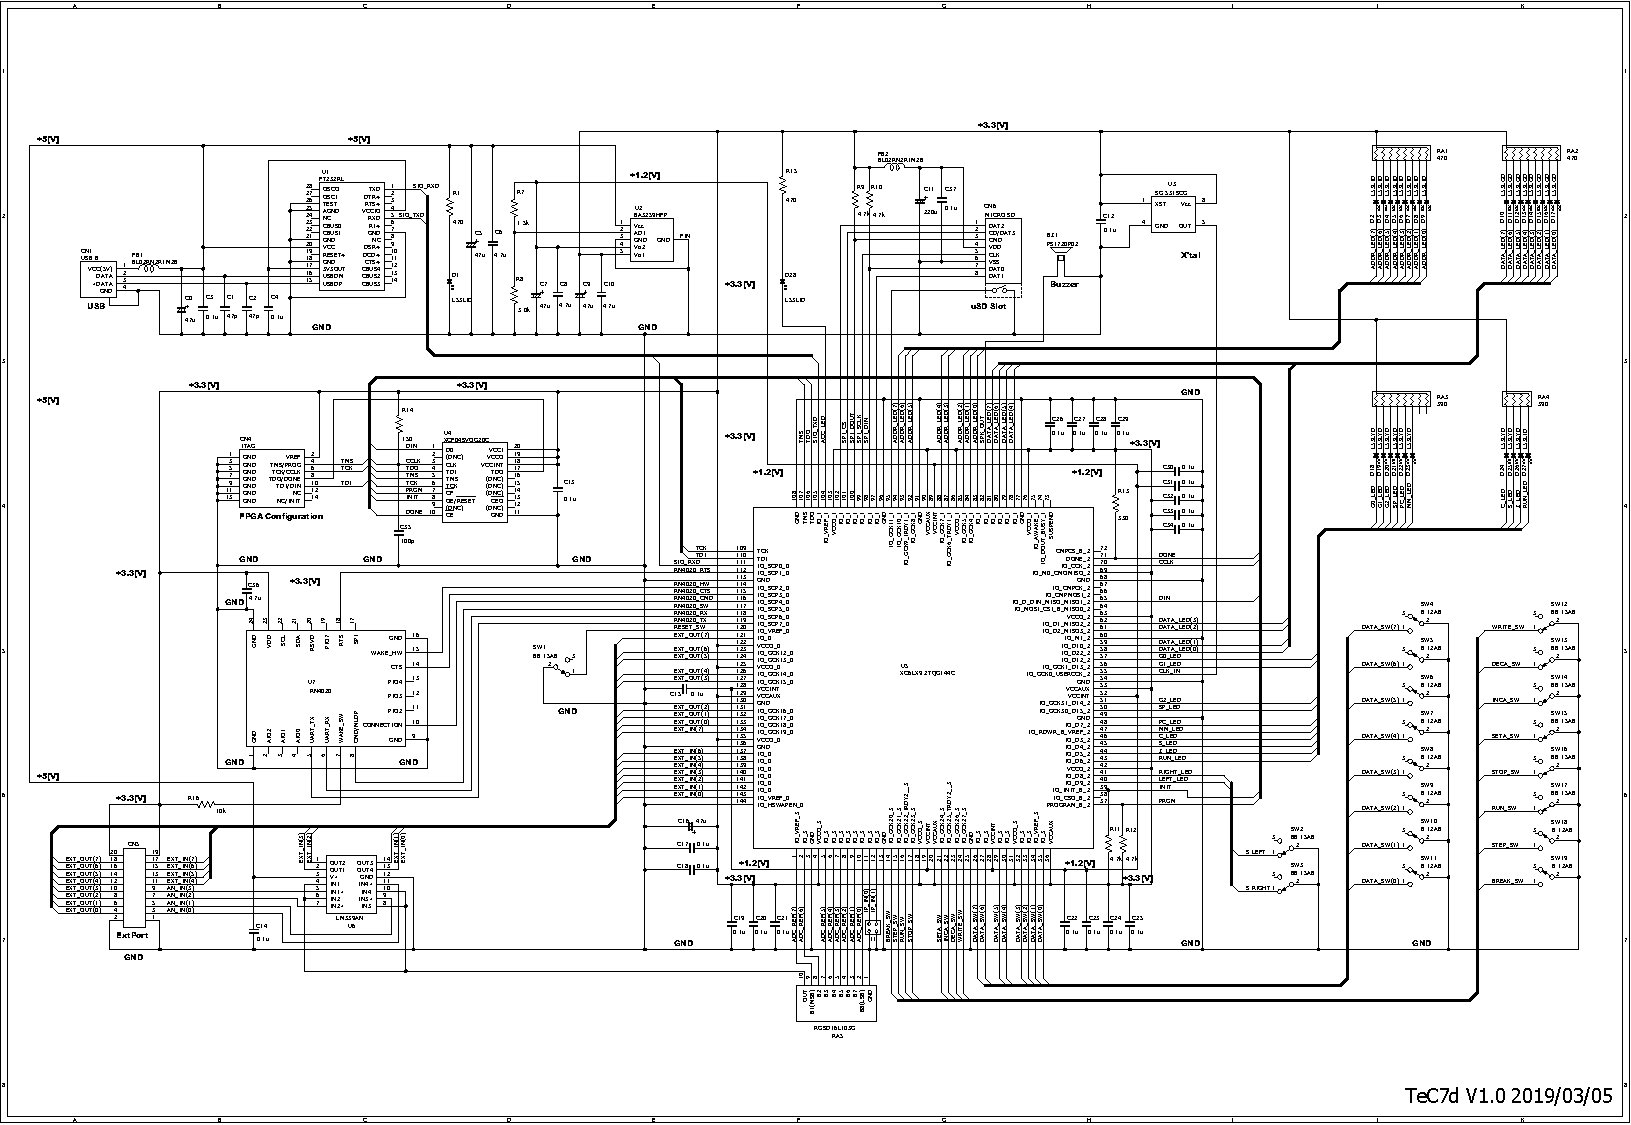
\includegraphics[angle=90,scale=0.85]{Fig/TeC7dPcb.pdf}
\end{myfig}

  % TaCの命令表・メモリマップ・I/Oマップ

%------------------------------------------------------------------------------
% 発行元
\backmatter
\pagestyle{empty}
\onecolumn
~
\vfill\vfill\vfill
\begin{center}
\fbox{\parbox{10cm}{ \vspace{0.3cm}
\large{\textbf{{\tecS} ハードウェアマニュアル \ver}} \\
\\
% 発行年月 2019年9月 \ver \\ %1.0.0
% 発行年月 2020年3月 \ver \\ %1.0.1
 発行年月 2022年3月 \ver \\ %2.0.0

 発  行 独立行政法人国立高等専門学校機構 \\
      徳山工業高等専門学校 \\
      情報電子工学科 重村哲至 \\
      〒745-8585 山口県周南市学園台3538 \\
      sigemura@tokuyama.ac.jp \\
}}
\end{center}
\vfill
\end{document}
